\documentclass[12pt,a4paper]{scrbook}
%--------------------------------------------------------------
\newcommand{\myItalianTitle}{Analisi del C.d.L. triennale in Informatica attraverso tecniche di Data Mining\xspace}
\newcommand{\myEnglishTitle}{Mining and Analysis on Computer Science Degree Course data\xspace}
\newcommand{\myDegree}{Corso di Laurea in Informatica\xspace}
\newcommand{\myName}{Simone Cipriani\xspace}
\newcommand{\myProf}{Donatella Merlini\xspace}
\newcommand{\myOtherProf}{Correlatore?\xspace}
\newcommand{\mySupervisor}{Supervisore?\xspace}
\newcommand{\myFaculty}{Scuola di Scienze Matematiche, Fisiche e Naturali\xspace}
\newcommand{\myUni}{\protect{Universit\`a degli Studi di Firenze}\xspace}
\newcommand{\myLocation}{Firenze\xspace}
\newcommand{\myTime}{Anno Accademico 2017-2018\xspace}
%--------------------------------------------------------------
\usepackage[italian]{babel}
\usepackage[utf8]{inputenc}
\usepackage[T1]{fontenc}
\usepackage[square,numbers]{natbib}
\usepackage[fleqn]{amsmath}
\usepackage{ellipsis}
\usepackage{listings}
\usepackage{subfig}
\usepackage{caption}
\usepackage{appendix}
\usepackage{siunitx}
\usepackage{dtk-logos} % just cause it's cool
%--------------------------------------------------------------
\usepackage{mod-classicthesis-ldpkg}
\usepackage[eulerchapternumbers,linedheaders,subfig,beramono,eulermath,parts,dottedtoc]{classicthesis}
%--------------------------------------------------------------
\newlength{\abcd}
\newcommand{\myfloatalign}{\centering}
\setlength{\extrarowheight}{3pt}
\captionsetup{format=hang,font=small}
%--------------------------------------------------------------
\usepackage{geometry}
\geometry{
	a4paper,
	bindingoffset = 1.5cm
}
\lstset{
  	frame=tb,
	language=Matlab,
  	aboveskip=3mm,
  	belowskip=3mm,
  	showstringspaces=false,
  	columns=flexible,
  	basicstyle={\small\ttfamily},
  	numbers=none,
  	breaklines=true,
  	breakatwhitespace=true,
  	tabsize=3
}
%--------------------------------------------------------------
\begin{document}
\frenchspacing
\raggedbottom
\pagenumbering{roman}
\pagestyle{plain}
%--------------------------------------------------------------
\begin{titlepage}
	\begin{center}
   	\large
      \hfill
      \vfill
      \begingroup
         
\includegraphics[scale=0.15]{logo/LOGO}\\
			\myFaculty \\
			\myDegree \\
			\vspace{0.5cm}
         \vspace{0.5cm}
         Tesi di Laurea
      \endgroup
      \vfill
      \vfill
      \begingroup
      	\color{Maroon}\spacedallcaps{\myItalianTitle} \\ $\ $\\ \spacedallcaps{\myEnglishTitle} \\ $\ $\\
	\bigskip
      \endgroup
      \vfill
      \vfill
            \spacedlowsmallcaps{\myName}
      \vfill
      \vfill
      Relatore: \emph{\myProf}\\
      \vfill
      \vfill
      \vfill
      \vfill
      \myTime
      \vfill
	\end{center}
\end{titlepage}
%--------------------------------------------------------------
   \newpage
	\thispagestyle{empty}
	\hfill
	\vfill
	\noindent\myName:
	\textit{\myItalianTitle,}
	\myDegree, \textcopyright\ \myTime


\pagestyle{scrheadings}
%--------------------------------------------------------------
\pagenumbering{arabic}
\tableofcontents
\listoffigures
\cleardoublepage
\thispagestyle{empty}
\begin{flushright}
\null\vspace{\stretch {1}}
\emph{"Inserire citazione" \break --- Inserire autore citazione} \vspace{\stretch{2}}\null
\end{flushright}
\cleardoublepage
%-------------------------------------------------------
\begin{frame}{Introduction}{What is Data Mining?}
%-------------------------------------------------------

\noindent\begin{centering}
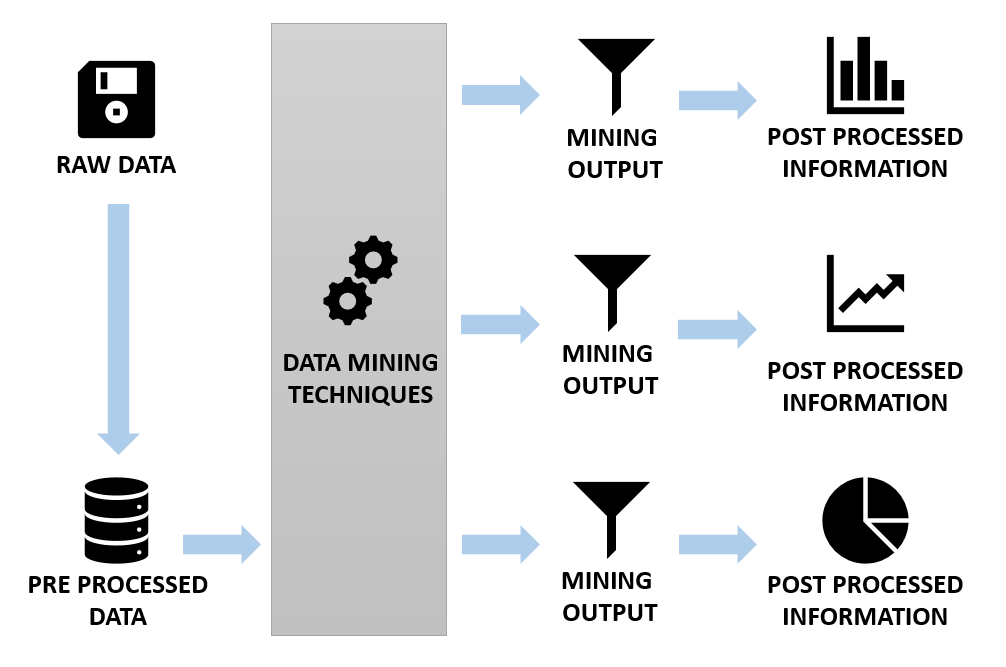
\includegraphics[scale=0.32]{img1_noback.png}
\end{centering}

\end{frame}

%-------------------------------------------------------
\begin{frame}{Introduction}{A general view about the Data Mining process}
%-------------------------------------------------------

    \centering\textit{What needs to be done?} \vspace{0,3cm}

	\begin{block}{}
		\begin{itemize}
			\item<1-> \textbf{Data Understanding}: analyze available raw data to \emph{understand} what can be extracted;
			\item<2-> \textbf{Preprocessing}: transform raw data into a \emph{minable} form, ready to be fed to the \emph{data mining algorithm};
			\item<3-> \textbf{Data Mining}: run the appropriate algorithm on the preprocessed data, to dig it for \emph{information};
			\item<4-> \textbf{Postprocessing}: display information in a human-friendly way, emphatizing what has beed dug with \emph{visualization technoques}.
		\end{itemize}
	\end{block}

\end{frame}

%-------------------------------------------------------
\begin{frame}{Introduction}{The choice of appropriate technologies}
%-------------------------------------------------------

	\centering\textit{Which technology should be employed?} \vspace{0,3cm}

	\begin{block}{}
	    \begin{itemize}
		    \item<1-> \alert{Data Processing} --- \textbf{MongoDB}: advanced \emph{dbms}, operating in the \emph{noSQL} paradigm.
		    \item<2-> \alert{Data Mining Algorithms} --- \textbf{Weka}: software which provide a \emph{framework} for running data mining algorithms.
			\item<3-> \alert{Visualization Techniques} \\
			--- \textbf{R language}: programming language with an extensive data visualization library; \\
			--- \textbf{Spreadsheets}: tabular data managing software, like Microsoft Excel and OpenOffice Calc.
	    \end{itemize}
    \end{block}

\end{frame}

\chapter{Dati Iniziali}
\label{ch:rawd}

In questo capitolo ci si soffermerà in quella che è una preliminare analisi dei dati iniziali a disposizione. Questi dati rappresentano il materiale grezzo dal quale \textit{estrarre} --- fare del \textit{mining}, come appunto il nome dell'attività suggerisce --- delle informazioni. \\

Usando come metafora una lavorazione meccanica, avere ben chiara la natura del materiale grezzo a disposizione consente di scegliere opportunamente gli utensili adatti per il lavoro da fare. Nel nostro caso, poter vantare di una comprensione generale di ciò che si ha a disposizione, potrà consentirci di scegliere le tecniche migliori per trarre il meglio dai dati iniziali. \\

\section{Carriera degli Studenti}

Una parte fondamentale dell'analisi descritta in questo lavoro è basata sul seguente data set, che contiene i dati riguardanti la produttività di tre coorti d'immatricolazione di studenti in un periodo di quattro anni. Più nel dettaglio, il dataset si compone di:

\begin{itemize}
	\item \textbf{coorte 2010}: studenti immatricolati nel 2010, carriera registrata fino agli appelli di \textbf{febbraio 2014}
	\item \textbf{coorte 2011}: studenti immatricolati nel 2011, carriera registrata fino agli appelli di \textbf{febbraio 2015}
	\item \textbf{coorte 2012}: studenti immatricolati nel 2012, carriera registrata fino agli appelli di \textbf{febbraio 2016}
	\item \textbf{coorte 2013}: studenti immatricolati nel 2013, carriera registrata fino agli appelli di \textbf{febbraio 2017}
\end{itemize}

\begin{figure}
    \centering
    \caption{Anni Accademici coperti dai dati a disposizione nel data set degli studenti}
    \label{1}
	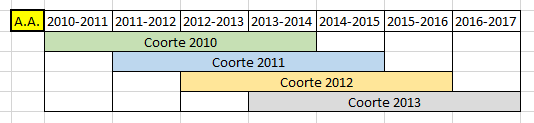
\includegraphics[scale=0.75]{../raw/stud_comp.png}
\end{figure}

Quindi, si ha a disposizione una finestra temporale di risultati ottenuti negli esami composta approssimativamente come indicato in Figura \ref{1}. Questo fatto porta ovviamente ad avere una mole d'informazioni più addensata nella parte centrale della nostra finestra temporale, avendo idealmente dati riguardanti gli esiti del maggior numero di corsi possibili solo per l'Anno Accademico 2013-2014. Tale aspetto sarà rilevante nell'interpretare i risultati di alcune analisi effettuate in seguito.

\subsection{Formato e Rappresentazione}

Il dataset è stato fornito in un unico file CSV, un formato \textit{plain text} facilmente manipolabile e interpretabile da un'ampia gamma di software. Esso si compone di una unica tabella, nella quale ogni tupla identifica uno studente, per il quale sono presenti attributi che descrivono la sua carriera universitaria nel periodo preso in esame. Oltre alle informazioni generali, quali ad esempio i risultati conseguiti nel test d'ingresso e il numero di crediti totali ottenuti nella finestra temporale esaminata, sono presenti attributi relativi alla data e al voto ottenuto in ciascun esame sostenuto. \\

Nel dettaglio, per ogni tupla rappresentante uno studente sono presenti le seguenti informazioni:

\begin{itemize}
	\item \textbf{Coorte} di immatricolazione: $$ \{2010, 2011, 2012, 2013\} $$
	\item Voto conseguito nel \textbf{test di ingresso}: $$ \{ x \in \mathbb{N} \text{ tale che } 0 \leq x \leq 25\} $$
	\item Voto ottenuto all'\textbf{esame di maturità}: $$ \{ x \in \mathbb{N} \text{ tale che } 60 \leq x \leq 100\} $$
	\item Tipo di \textbf{scuola superiore} frequentata: $$ \{LS, LC, IT, TC, IP, AL \} $$ che rappresentano rispettivamente le seguenti categorie di scuola superiore: Liceo Scientifico, Liceo Classico, Istituto Tecnico, Istituto Commerciale, Istituto Professionale, Altro
	\item \textbf{Crediti totali} ottenuti: $$ \{ x \in \mathbb{N} \text{ tale che } 0 \leq x \leq 180\} $$
	\item \textbf{Crediti} ottenuti da esami \textbf{con voto}: $$ \{ x \in \mathbb{N} \text{ tale che } 0 \leq x \leq 159\} $$
	\item \textbf{Voto medio} ottenuto negli esami: $$ \{ x \in \mathbb{N} \text{ tale che } 18 \leq x \leq 31 \text { con 31 indicante il 30 con lode}\} $$
	\item \textbf{Voto} ottenuto in un \textbf{certo esame}: $$ \{ x \in \mathbb{N} \text{ tale che } 18 \leq x \leq 31 \text { con 31 indicante il 30 con lode}\} $$
	\item \textbf{Data} in cui è stato sostenuto quell'esame: $$ \text{data in formato }MM/GG/YYYY $$
\end{itemize}

Di tutte queste informazioni, solo parte di esse sono state utilizzate in qualche analisi di \textit{data mining}, come si vedrà meglio nelle sezioni successive.

\subsection{Mole di dati}

Il dataset si compone di 208 record, ognuno dei quali ha 47 attributi. Il file che lo memorizza pesa circa 45 kb. Non si può quindi parlare propriamente di \textit{big data} in questo caso.

\section{Valutazione degli Insegnamenti}

Al fine d'integrare i dati precedenti ponendo l'attenzione sui vari corsi che compongono il Corso di Laurea, sono stati forniti i dati relativi alla valutazione dei corsi di studi da parte degli studenti. Questi dati sono ottenuti da questionari anonimi, che devono essere obbligatoriamente compilati prima di potersi prenotare per un esame. I risultati sono poi divulgati in forma aggregata, garantendo così l'anonimato dello studente. A ogni domanda lo studente ha potuto rispondere indicando un valore compreso fra zero e dieci, con zero a indicare una risposta totalmente negativa e dieci a indicare invece una risposta totalmente positiva.\\

Volendo scendere in un maggior dettaglio, sono stati forniti i dati riguardanti i seguenti anni accademici:

\begin{itemize}
	\item 2010-2011
	\item 2011-2012
	\item 2012-2013
	\item 2013-2014
	\item 2014-2015
	\item 2015-2016
	\item 2016-2017
\end{itemize}

Come si può facilmente notare, la finestra temporale coperta da questi dati va a combaciare con quella trattata dal dataset relativo alla carriera degli studenti. Questo aspetto fondamentale ha permesso di effettuare una operazione di \textit{join} fra i due dataset a disposizione, che verrà in seguito descritta nella sezione dedicata al \textit{preprocessing}.

\subsection{Formato e Rappresentazione}

Il dataset è stato fornito in sette diversi file CSV, uno per ogni anno accademico per il quale sono state espresse valutazioni dei relativi corsi. In ogni file si rappresenta una tabella le cui tuple identificano una valutazione relativa a un particolare aspetto di un corso, riportata ovviamente in forma aggregata. \\

\noindent Nel particolare, ogni record di questo tipo di tabelle è identificato dai seguenti campi, che agiscono come chiave:

\begin{itemize}
	\item \textbf{Codice identificativo}: stringa alfanumerica che identifica univocamente l'esame oggetto di valutazione all'interno del Corso di Laurea in esame.
	\item \textbf{Nome del corso}: stringa descrittiva che identifica il Corso di Laurea \textit{(in questo caso, "INFORMATICA")}.
	\item \textbf{Tipo di corso}: stringa descrittiva che identifica il tipo di Corso di Laurea \textit{(in questo caso, "Triennale")}.
	\item \textbf{Insegnamento}: stringa descrittiva che identifica l'esame oggetto di valutazione.
	\item \textbf{Docente/i}: stringa descrittiva che identifica il docente che ha tenuto il corso e svolto l'esame.
	\item \textbf{Paragrafo}: stringa descrittiva che identifica il paragrafo del questionario di valutazione.
	\item \textbf{Q}: stringa alfanumerica che identifica univocamente la domanda posta.
	\item \textbf{Quesito}: stringa descrittiva contenente il testo della domanda posta allo studente.
\end{itemize}

\noindent  Si notiche ilcampo riguardante il docente ne riporta originariamente nome e cognome per esteso. Per salvaguardarne la privacy, i valori di questo campo sono stati sostituiti con le loro immagini tramite una funzione di \textit{hash}, preservando l'unicità del valore ma nascondendo l'effettiva identità del docente. \\

A ogni tupla, identificata dai valori dei campi precedentemente descritti, corrispondono queste informazioni:

\begin{itemize}
	\item \textbf{P1, P2}: $ \{ x \in \mathbb{R} \text{ tale che } 0 \leq x \leq 100 \} $  percentuali rispettivamente di risposte sufficienti ($ \geq 6$) e insufficienti ($ < 6$).
	\item \textbf{Media}:  $ \{ x \in \mathbb{R} \text{ tale che } 0 \leq x \leq 10 \} $ media artimetica delle valutazioni ottenute.
	\item \textbf{Deviazione Standard}:  $ \{ x \in \mathbb{R} \text{ tale che } x \geq 0\} $ scarto quadratico medio delle singole valutazioni.
	\item \textbf{N}:  $ \{ x \in \mathbb{N} \text{ tale che } x \geq 6\} $ quantità di valutazioni utilizzate per calcolar ei precedenti valori.
\end{itemize}

Come è possibile intuire, molti di questi attributi sono inutili o ridondanti. Il compito di valutarne l'utilità ed eventualmente di sfoltirli sarà svolto nella fase di \textit{preprocessing}.

\subsection{Mole di dati}

I sette file forniti contengono complessivamente 2594 record, ognuno dei quali ha 13 attributi. Anche riguardo a questo dataset, non si può usare propriamente la denominazione \textit{big data}.\\

In ogni caso, visto che le quantità in gioco non sono comunque piccole, in una eventuale \textit{join} con il dataset precedente occorrerà fare particolare attenzione a non moltiplicare la quantità di record generando ridondanze, in quanto un simile errore potrebbe facilmente rendere l'insieme di dati risultante intrattabile.

\section{Conclusioni dell'Analisi dei Dati Iniziali}

Dopo aver esaminato attentamente i due dataset a disposizione, si può immediatamente affermare che il focus principale dell'analisi dovrà essere posto sui singoli corsi, per i quali si hanno molte informazioni di vario genere. \\

Volendo quindi sintetizzare quanto è stato possibile capire dall'analisi presentata in questa sezione, elaborandolo nell'ottica appena acquisita, si può riassumere la descrizione del materiale a nostra disposizione in due semplici punti:

\begin{itemize}
	\item risultati dei singoli studenti
	\item aggregazioni delle risposte ai questionari di valutazione dei corsi
\end{itemize}

Oltre a effettuare analisi sui singoli insiemi di dati, si potrà immaginare di doverli in qualche modo unire per incrociarne le informazione e trovare, possibilmente, correlazioni interessanti. Si può quindi dire che la sfida più impegnativa della prossima fase, il \textit{preprocessing}, riguardi la messa in relazione di dati aventi natura diversa. \\

Di pari passo a essa, sarà portata avanti una fase di \textit{data understanding}. Sarà utile per affinare la comprensione di quanto si è appena mostrato e per decidere il tipo di tecniche di \textit{data mining} da utilizzare sulla mole di dati a disposizione.

\chapter{Technology Stack}

La scelta della tecnologia da impiegare è un aspetto fondamentale di ogni progetto, e questo chiaramente non fa eccezione. \\

Molti testi --- fra cui uno dei preferiti dall'autore\footnote{Si tratta di \cite{pragmatic}, un libro estremamente interessante, oltre che essenziale come spunto di riflessione per lo sviluppo personale e professionale di ogni informatico che osi definirsi programmatore.} --- hanno proposto analogie fra gli utensili di un artigiano e gli strumenti software di un qualaunque utlizzatore informatico. Sull'onda di questa metafora, una lima non adatta al tipo di materiale che si intende lavorare non potrà mai garantire risultati eccellenti, indipendentemente dalla bravuta dell'artigiano stesso. \\

Appare chiaro che una scelta sbagliata di tecnologie da utilizzare può condizionare negativamente l'esito di un qualaunque lavoro, pertanto occorre prestare particolare attenzione nel decidere quale tecnologia impiegare per raggiungere lo scopo.

\section{Strumenti Necessari}

    Messi da parte i vaneggiamenti poetici, all'atto pratico è evidente che gli strumenti di cui l'analisi ha bisogno sono in realtà pochi e piuttosto comuni:

    \begin{itemize}
        \item abbiamo a che fare con una certa quantità di dati $\rightarrow$ servirà un \textit{Data Base Management System}.
        \item occorre avere una comprensione generale dei dati $\rightarrow$ occorrerà un software che permetta di usare \textit{tecniche di visualizzazione}.
        \item dobbiamo lanciare degli algoritmi di \textit{data mining} $\rightarrow$ abbiamo bisogno di un software che li implementi.
    \end{itemize}

    Tutto questo è facilmente ottenibile impiegando gli strumenti che saranno descritti nelle prossime sezioni.

\section{Data Base Management System: MongoDB}

    \begin{figure}
        \centering
        \caption{logo del DBMS MongoDB}
        \label{mongodb_logo}
    	
\includegraphics[scale=0.70]{img/mongodb.png}
    \end{figure}

    La scelta del Data Base Management System è stata quella che ha impattato più di tutte il tipo di lavoro che è stato necessario fare.

    \subsection{La scelta di MongoDB}
    
        Sono state valutati principalmente due \textit{DBMS} candidati, entrambi \textit{open source}:

        \begin{itemize}
            \item \textbf{MySQL}, un \textit{DBMS} relazionale, rodato e ormai \textit{staple} nella manipolazione dati
            \item \textbf{MongoDB}, un \textit{DBMS} di nuova generazione che adotta invece il paradigma \textit{NoSQL} 
        \end{itemize}

        I dati che si hanno a disposizione sono in forma ovviamente relazionale --- cioè, sono tabelle. Utilizzare \textit{MySQL} potrebbe sembrare quindi una scelta tanto solida quanto ovvia, ma sul piano prestazionale il \textit{modello a documenti} di \textit{MongoDB} risulta sensibilmente più efficiente nel manipolare grandi quantità di dati molto diversi fra loro. \\

        La decisione che è stata infine presa --- \textit{utilizzare MongoDB} --- ha tenuto conto anche del valore didattico che ha l'imparare un nuovo paradigma di memorizzazione dati che trascende il classico modello relazionale.

    \subsection{Caratteristiche di MongoDB}

        Come si può banalmente leggere in \cite{mongowiki}: \\
        
        "\textbf{MongoDB} \textit{(da "humongous", enorme)} è un DBMS non relazionale, orientato ai documenti. Classificato come un database di tipo \textbf{NoSQL}, MongoDB si allontana dalla struttura tradizionale basata su tabelle dei database relazionali in favore di \textbf{documenti in stile JSON} con schema dinamico (MongoDB chiama il formato BSON), rendendo l'integrazione di dati di alcuni tipi di applicazioni più facile e veloce." \\

        La società MongoDB Inc mette a disposizione liberamente e gratuitamente una buona documentazione in \cite{mongodb}, la quale contiene tutte le informazioni necessarie per utilizzare almeglio il DBMS da loro sviluppato. 

        Oltre alla sua \textit{shell}, MongoDB espone delle \textit{API} per i principali linguaggi di programmazione. Questo aspetto è tornato molto utile per specificare le operazioni di \textit{preprocessing} in un linguaggio familiare e più facilmente gestibile del dialetto di Javascript nativo di MongoDB.

\section{Interazione col DBMS: Python}

    \begin{figure}
        \centering
        \caption{logo del linguaggio di programmazione Python}
        \label{python_logo}
    	
\includegraphics[scale=0.1]{img/python.png}
    \end{figure}

    A proposito di quando detto alla fine della sezione precedente, il linguaggio scelto è stato \textbf{Python}. Come si può leggere direttamente da \cite{pywiki}:\\

    "\textit{Python} è un linguaggio multi-paradigma, che ha tra i principali obiettivi \textit{dinamicità}, \textit{semplicità} e \textit{flessibilità}. Supporta il paradigma object oriented, la programmazione strutturata e molte caratteristiche di programmazione funzionale e riflessione." \\

    Il linguaggio Python ha una estesa e approfondita documentazione, messa a disposizione direttamente dalla Python Software Foundation in \cite{python}.

    \subsection{API per MongoDB: pymongo}

        \begin{figure}
            \centering
            \caption{schema riassuntivo del modello di lavoro con \textbf{pymongo}}
            \label{pymongo_logo}
    	    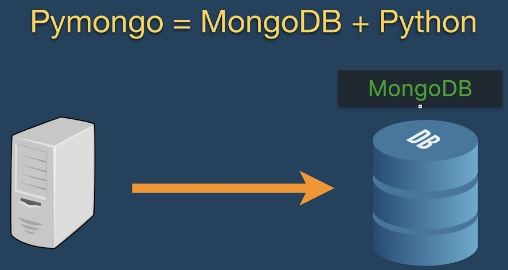
\includegraphics[scale=0.75]{img/pymongo.png}
        \end{figure}

        Una sintetica ma tremendamente efficace descrizione di che cosa è \textbf{pymongo} si può trovare direttamente nella sua documentazione, in \cite{pymongo}:\\

        "PyMongo is a Python distribution containing tools for working with MongoDB, and is the recommended way to work with MongoDB from Python." \\

        Ovvero: \\

        "PyMongo è una distribuzione di Python che contiene degli strumenti per lavorare con MongoDB, ed è la maniera raccomandata per avere a che fare con MongoDB da Python." \\








\lstset{language=R,
    basicstyle=\small\ttfamily,
    stringstyle=\color{gray},
    otherkeywords={0,1,2,3,4,5,6,7,8,9},
    morekeywords={TRUE,FALSE},
    deletekeywords={data,frame,length,as,character},
    keywordstyle=\color{blue},
    commentstyle=\color{gray},
}

\chapter{Data Understanding Preliminare}

La fase che verrà descritta in seguito è fra le più delicate di tutto il processo di \textit{data mining}. Da essa dipende la buona riuscita o meno dell'intera attività di estrazione d'informazioni. Come appare quindi naturale, è stata dedicata a essa una particolare attenzione.

    \section{Introduzione al Data Understanding}

        \subsection{Scopo dell'Attività}

            Perché occorre spendere del tempo per perpetrare un'estesa fase di \textit{data understanding}? \\

            Banalmente, l'obiettivo principale che ci si prefigge è quello di ottenere una chiara visione d'insieme sui dati che si hanno a disposizione. In questo modo, si sarà in grado di prendere decisioni oculate per quanto riguarda il da farsi nei successivi passi di questa analisi. Si prenda ad esempio l'attività di \textit{preprocessing}: sintetizzando al massimo, possiamo dire che si tratta di lavorare dei dati grezzi al fine di renderli adatti a essere processati da certi algoritmi. L'ovvia implicazione è che occorre avere ben chiaro in anticipo quali algoritmi sarà opportuno lanciare, fatto che a sua volta implica la necessità di conoscere quali informazioni si intende estrarre dai dati grezzi a disposizione. \\

            Questo aspetto rende necessario far precedere a quello che è, usando una metafora nell'ambito meccanico, l'attività di sgrossatura dei dati grezzi una fase di \textit{data understanding}. \\

            In questa sezione, quindi, si punterà a capire a fondo la natura dei dati al fine d'intuire che cosa sia possibile trarne.

        \subsection{Metodi e Strumenti}

            L'attività di \textit{data understanding} può essere svolta in molti modi, non essendoci delle regole fisse che la disciplinano rigidamente. Si può azzardare che le risorse più importanti alle quali si può attingere in questo ambito sono, piuttosto romanticamente, l'intuito e la fantasia dei \textit{data scientist} coinvolti nel progetto. Fuori di metafora, è chiaro che non esistano procedure che indichino univocamente le informazioni che è possibile ricavare su un dato insieme di dati. Perciò, quello che occorre fare è sfruttare dei metodi che riassumano i dati per poterli apprezzare nel loro insieme. \\

            Gli strumenti più adatti per poter ottenere una visione d'insieme sull'intera mole di dati sono, senza ombra di dubbio, le varie \textit{tecniche di visualizzazione} esistenti. Il loro utilizzo è stato permesso da software quali \textbf{R} e \textbf{Weka}, oltre che da più comuni \textit{spreadsheet} forniti da suite di programmi da ufficio. \footnote{Per un maggior dettaglio, si consulti il capitolo riguardo alla \textit{technology stack} impiegata per la realizzazione di questo progetto.}

    \section{Data Set: Produttività degli Studenti}

        Senza ombra di dubbio questa porzione di dati rappresenta la più significativa dell'intero lotto a disposizione per questa analisi. \\

        Si è quindi optato per utilizzare il software \textbf{R}, in quanto consente d'impiegare efficientemente un gran numero di approfondite tecniche di visualizzazione. Tuttavia, la potenza e la flessibilità offerte da questo tipo di strumento si pagano con la necessita di dedicare un minimo di attenzione all'importazione del data set in quell'ambiente di lavoro. \\

        In senso pratico, questo si traduce nel lanciare del codice analogo \footnotesize{--- non identico: sono stati accorciati i percorsi ---}\normalsize\ a quanto mostrato di seguito prima di poter effettuare qualunque altra operazione.

        \newpage

        \begin{lstlisting}
        # set the repo root path before importing data!!!
        setwd("C:/a/path/to/somewhere")
        students <- read.csv("raw/prod_stud.csv")

        # gather some info about the imported data set
        str(students)

        # ADJUST DATA ATTRIBUTES 
        # convert "coorte" to nominal by making it a factor 
        students[, c(1)] <- sapply(students[, c(1)], factor)

        # ok, let's take a look at it now
        str(students)
        summary(students)
        \end{lstlisting}

        In ogni caso, dato l’elevato numero degli attributi del data set, è stato necessario prendere delle decisioni relative a cosa visualizzare – e con quale tecnica. Le scelte sono state ovviamente compiute su base intuitiva, a seguito di un’analisi sommaria delle caratteristiche del data set. \\

        È stato quindi deciso di effettuare una ricerca visiva di correlazioni fra valori di attributi relativi a:

        \begin{itemize}
            \item prestazioni generali durante tutto il periodo esaminato
            \item prestazioni nei singoli esami
            \item risultati di gruppi di esami
        \end{itemize}

        \subsection{Prestazioni Generali degli Studenti}

            Lo script \textbf{R} che segue disegna dei grafci di dispersione su coppie di attributi relativi alle prestazioni generali degli studenti. Lo scopo è quello di individuare visivamente delle correlazioni significative fra questi attributi.\\

            \begin{lstlisting}
            colors <- c("blue","red", "green", "orange")
            coorte_labels <- students[,1]
            coorte_colors <- colors[as.numeric(coorte_labels)]
            library(seriation)
            
            # general attributes
            students_subset1 <- students[,-c(1, 6 : 45)]
            pairs(students_subset1, col = coorte_colors,lower.panel = 	NULL,cex.labelsiris=2, pch=19, cex = 1.2)
            par(xpd = TRUE)
            legend(x = 0.05, y = 0.4, cex = 1,legend = 	as.character(levels(coorte_labels)),fill = unique(coorte_colors))
            par(xpd = NA)
            \end{lstlisting}

            \begin{figure}
                \centering
                \caption{grafico di dispersione su attributi generali}
                \label{fig1}
            	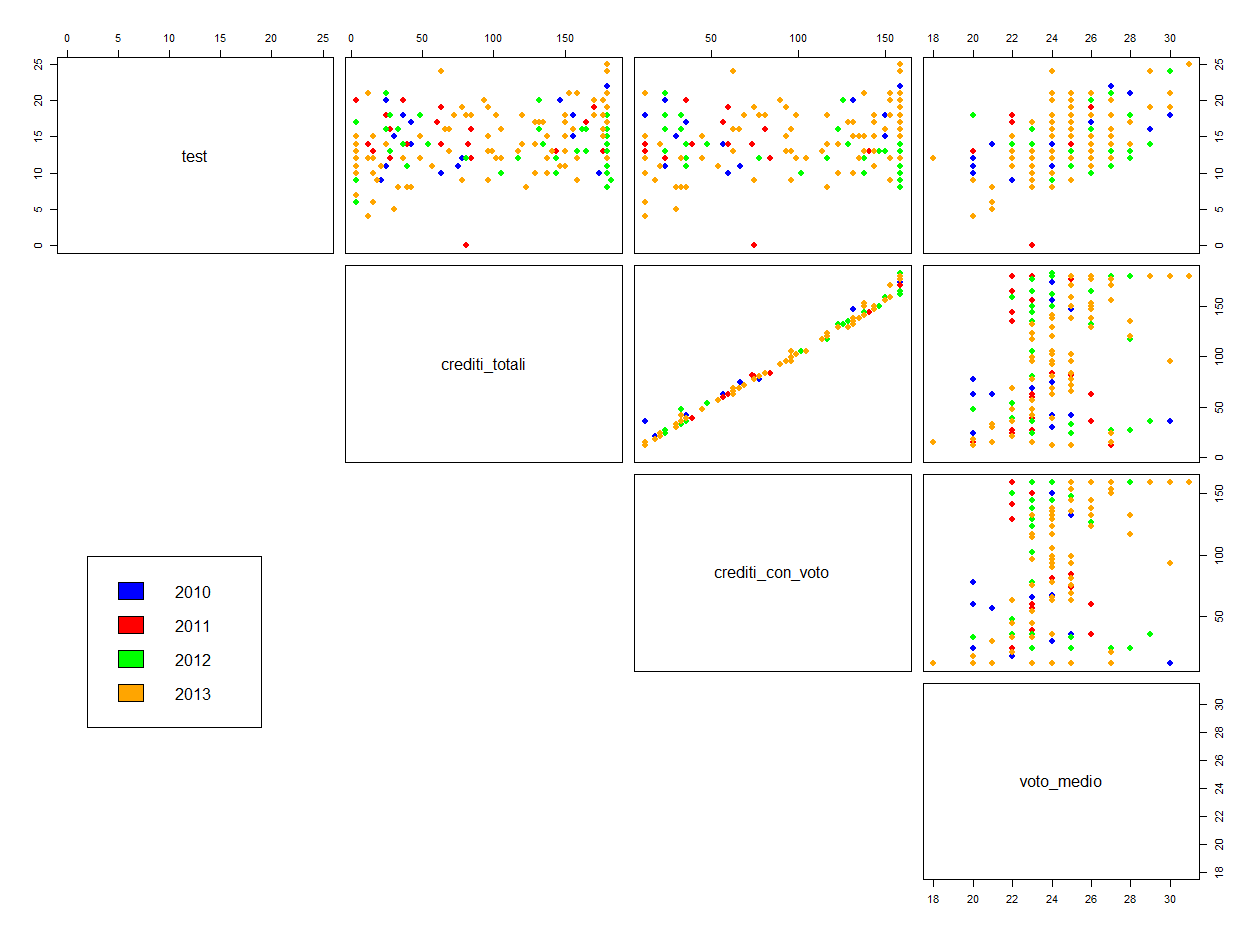
\includegraphics[scale=0.32]{img/scatter_plot_1_gen.png}
            \end{figure}

            Come si può vedere sul grafico generato dallo script --- mostrato in Figura \ref{fig1} --- esistono varie correlazioni fra gli attributi considerati. Nel merito, la relazione fra le quantità \textit{crediti totali} e \textit{crediti con voto} è tanto palese quanto banale: il primo ammontare contiene il secondo, e la loro differenza è minima. Appare invece più interessante quello che accade fra altre coppie di attributi:

            \begin{itemize}
                \item punteggio del test di ingresso e valore atteso del voto 
                \item quantità di crediti ottenuti e valore atteso del voto
            \end{itemize}

            Si ritiene quindi opportuno realizzare dei grafici che abbiano un maggior livello di dettaglio su questi aspetti.

            \begin{figure}
                \centering
                \caption{grafico di dispersione su voto medio e test di ingresso}
                \label{fig2}
            	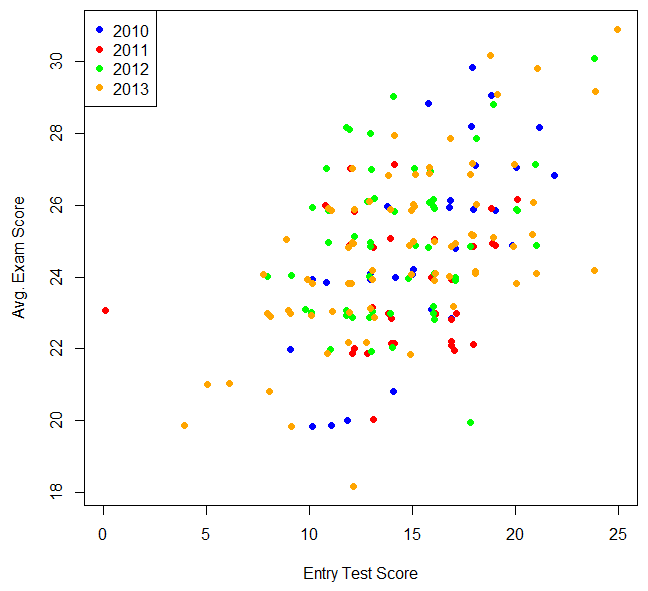
\includegraphics[scale=0.5]{img/scatter_plot_2.png}
            \end{figure}

            \begin{figure}
                \centering
                \caption{grafico di dispersione su voto medio e C.F.U. ottenuti}
                \label{fig3}
            	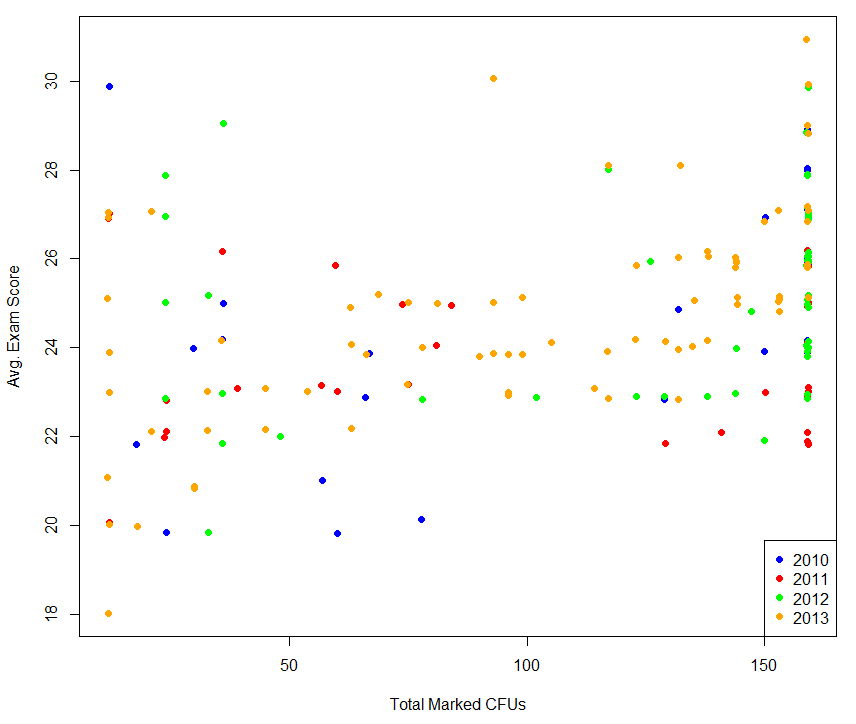
\includegraphics[scale=0.40]{img/scatter_plot_3.png}
            \end{figure}

            Come risulta dalla Figura \ref{fig2}, si potrebbe speculare che esista una correlazione lineare fra i due attributi: gli studenti che conseguono un punteggio alto nel test di ingresso sono più propensi ad ottenere voti alti negli esami. \\

            Per quanto riguarda invece la Figura \ref{fig3}, fra gli studenti che hanno conseguiti tutti i crediti si può notare una consistente densità nella fascia che va circa dal ventidue al ventinove. Si può anche notare una assenza di voti medi inferiori al 22 fra coloro che hanno conseguito più di 100 CFU. Un altro aspetto che potrebbe rivelarsi interessante è che, fra la coorte di studenti del 2013, vari studenti hanno conseguito un solo esame con un voto superiore al 20. \\

            Viste le possibili informazioni che sembra possibile estrarre, si è deciso d'insistere sull’analisi visiva degli attributi \textit{voto medio} e \textit{numero totale di crediti}. Sono stati quindi realizzati dei diagrammi a scatola e baffi con il seguente script \textbf{R}: 

            \begin{lstlisting}
            boxplot(students[,4]~students[,1],data = students,xlab="Total Marked CFU",col=colors)
            boxplot(students[,5]~students[,1],data = students,xlab="Avg. Exam Score",col=colors)
            \end{lstlisting}

            \begin{figure}
                \centering
                \caption{diagramma a scatole e baffi sull'attributo \textit{numero totale di crediti}}
                \label{boxplot1}
            	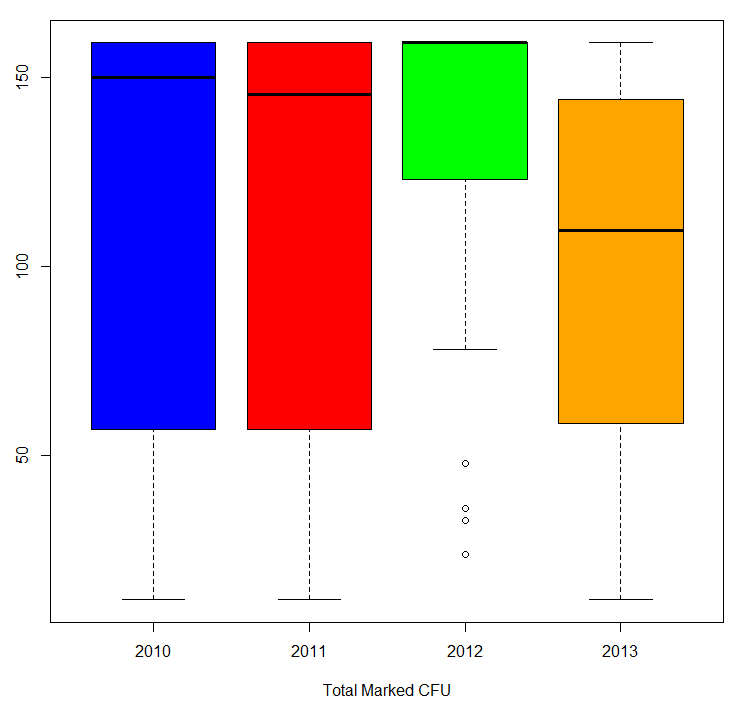
\includegraphics[scale=0.5]{img/box_plot_1.png}
            \end{figure}

            \begin{figure}
                \centering
                \caption{diagramma a scatole e baffi sull'attributo \textit{voto medio}}
                \label{boxplot2}
            	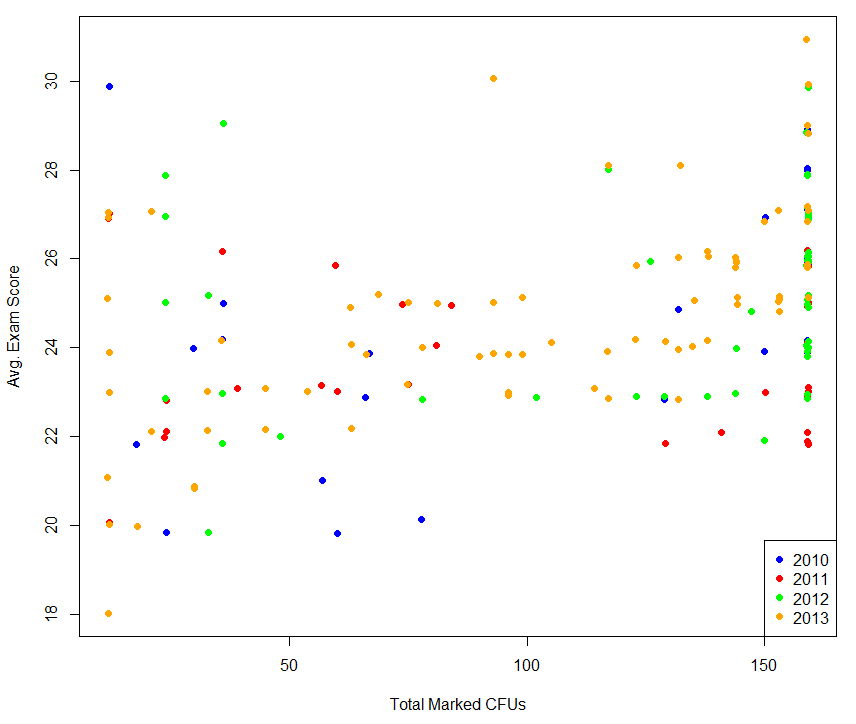
\includegraphics[scale=0.5]{img/scatter_plot_3.png}
            \end{figure}

            Riguardo al diagramma in Figura \ref{boxplot1}, si noti come gli immatricolati nelle annate 2010 e 2011 hanno prestazioni molto simili sul fronte dei crediti conseguiti. La coorte 2012 risulta la migliore, avendo addirittura per mediana il massimo ammontare di crediti ottenibili\footnote{non si ignorino però le istanze considerate \textit{outliers} dall’algoritmo!}, mentre gli studenti immatricolati nel 2013 sono stati i meno performanti.

            Nel caso invece del voto medio, rappresentato in Figura \ref{boxplot2}, si evidenzia solo un leggero peggioramento negli immatricolati nel 2011 rispetti alle altre coorti di studenti. Sono degni di attenzione anche i due \textit{outliers} nella coorte 2013.

        \subsection{Prestazioni degli Studenti su Gruppi di Esami}

            Una scelta significativa nell’ambito di questa fase è stata la suddivisione degli esami in vari gruppi. Si è cercato di raggruppare intuitivamente degli esami i cui risultati potrebbero essere correlati in qualche modo. L’ovvio rischio che si è scelto di correre è quello di non notare correlazioni che esistono, ma che non sono intuitive. \\

            La suddivisione più sensata è sembrata essere la seguente:

            \begin{itemize}
                \item esami del primo anno
                \item esami su argomenti principalmente informatici
                \item esami su argomenti principalmente matematici
            \end{itemize}

            \subsubsection{Esami del primo anno}

                Il seguente script \textbf{R} ha generato i grafici di dispersione, le matrici di correlazione e di deviazione standard utilizzate per l’analisi visiva del gruppo di esami del primo anno. Per gli altri gruppi di esami, gli script sono stati molto simili.

                \begin{lstlisting}
                # general first year exams performances
                students_subset2 <- students[,-c(1 : 5, 7, 9, 11, 13, 15 : 45)]
                pairs(students_subset2, col = coorte_colors,lower.panel = NULL,cex.labelsiris=2, 	pch=19, cex = 1.2)
                par(xpd = TRUE)
                legend(x = 0.05, y = 0.4, cex = 1,legend = as.character(levels(coorte_labels)),fill 	= unique(coorte_colors))
                par(xpd = NA)
                
                students_scaled <- scale(students_subset2)
                pimage(students_scaled,ylab="Students",main="Standard Deviations from Mean Mark")
                
                matrix <- as.matrix(students_scaled)
                cm <- cor(t(matrix), method="pearson")
                pimage(cm,main="Correlation Matrix considering 1st Year exams", xlab="Students", 	ylab="Students",zlim = c(-1,1),col = bluered(50))
                \end{lstlisting}

                \begin{figure}
                    \centering
                    \caption{grafico di dispersione relativo agli esami del primo anno}
                    \label{esami1anno_sp}
                	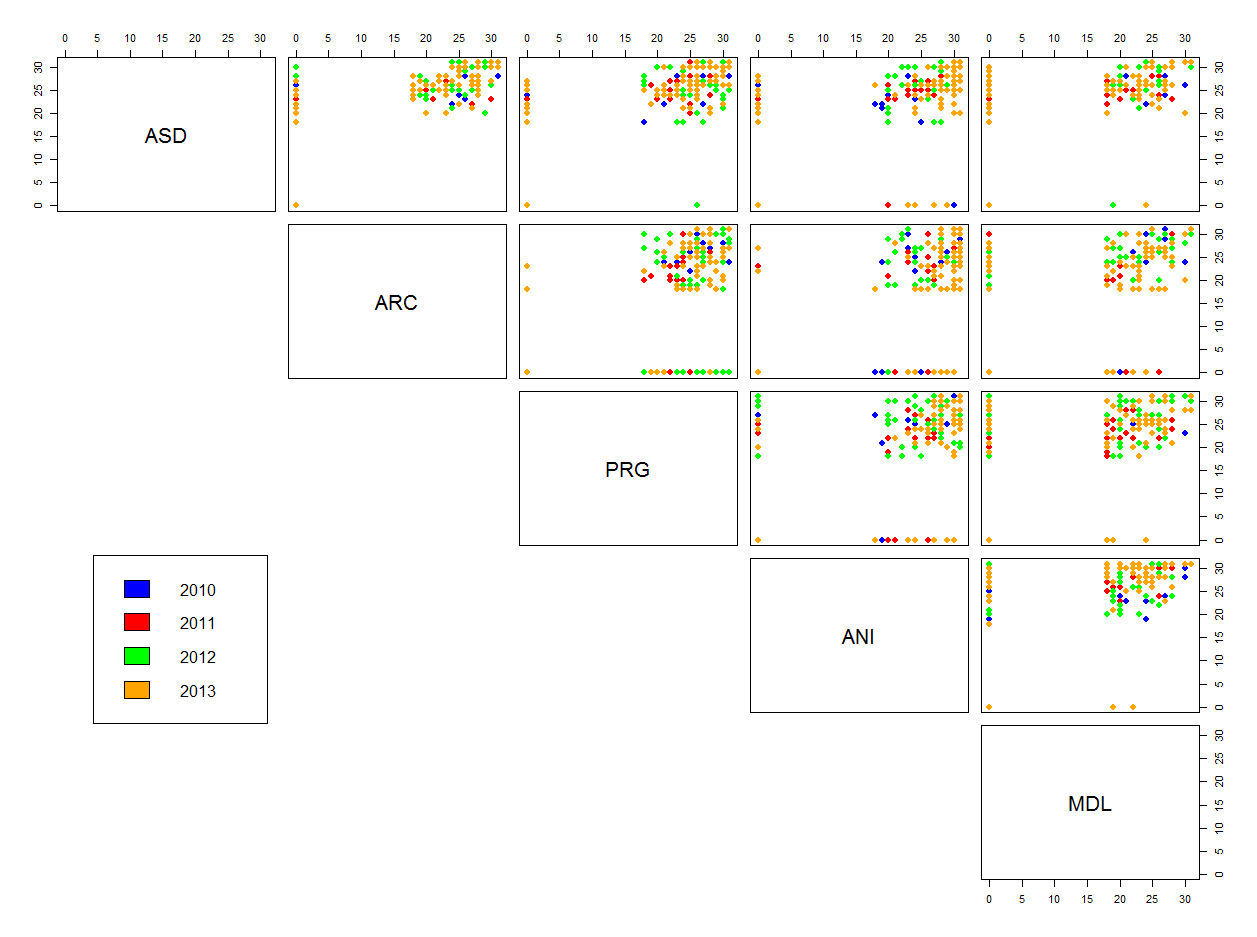
\includegraphics[scale=0.32]{img/scatter_plot_4_gen.png}
                \end{figure}

                Dall’analisi visiva del grafico di dispersione in Figura \ref{esami1anno_sp} non si è stati in grado di concludere molto di concreto. Eppure si ritiene possibile che qualche informazione interessante si possa nascondere dentro l’insieme di dati degli esami del primo anno; occorre scendere nel dettaglio. A questo proposito, sono state realizzate le matrici mostrate nelle Figure \ref{esami1anno_corr} e \ref{esami1anno_stddev}.

                \begin{figure}
                    \centering
                    \caption{matrice di correlazione sugli esami del primo anno}
                    \label{esami1anno_corr}
                	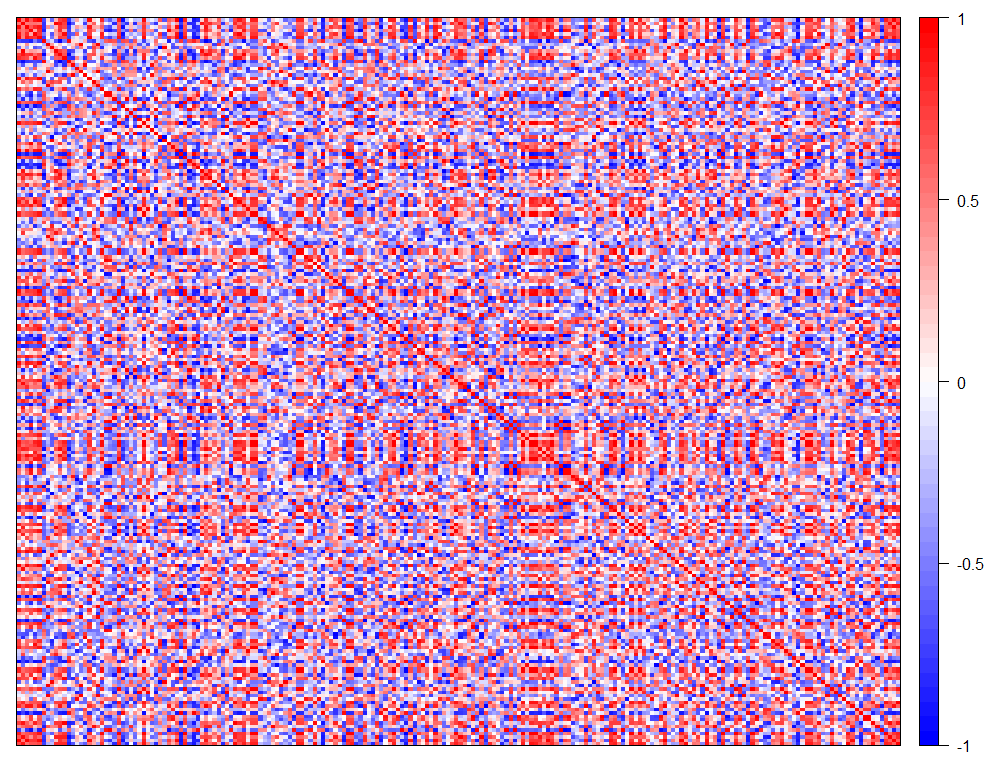
\includegraphics[scale=0.32]{img/corr_matrix_1.png}
                \end{figure}

                \begin{figure}
                    \centering
                    \caption{matrice dello scarto quadratico medio sugli esami del primo anno}
                    \label{esami1anno_stddev}
                	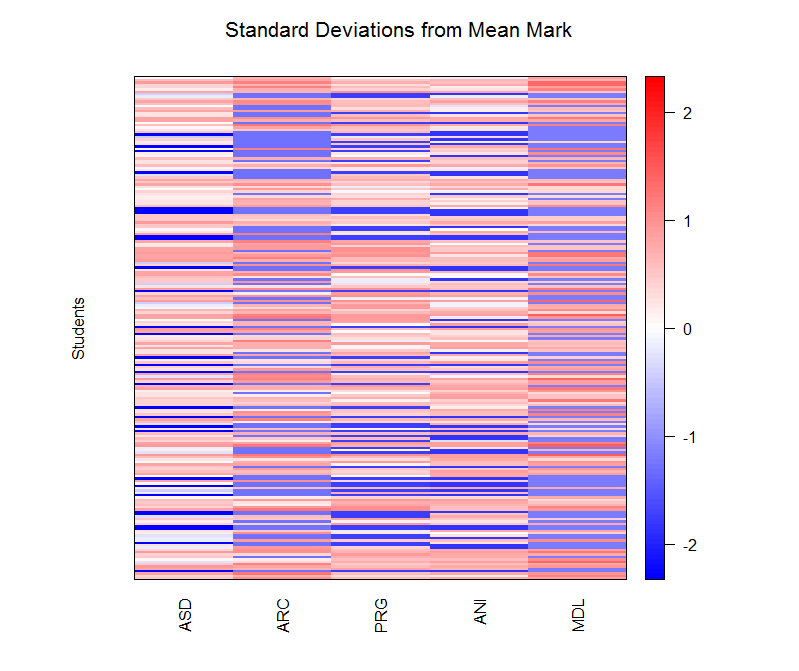
\includegraphics[scale=0.5]{img/std_dev_matrix_1.png}
                \end{figure}

                Per quanto riguarda invece quanto mostrato in Figura \ref{esami1anno_corr}, come misura di correlazione è stata scelta la \textit{correlazione di Pearson}, ricercando quindi relazioni monotone. Si nota un accenno di trama in due punti, sintomo di similarità fra due fasce di studenti. Quesrto può far pensare che potrebbe essere possibile individuarle con algoritmi di \textit{clustering}.

                Osservando invece la Figura \ref{esami1anno_stddev}, si può evidenziare che i colori più tiepidi della deviazione standard per gli esami di \textit{Matematica Discreta e Logica} e \textit{Architetture degli Elaboratori} stanno ad indicare una minore tendenza a discostarsi dal voto medio. Perché studenti di vari anni tendono a convergere verso lo stesso voto in quei due esami? Per rispondere a questa domanda, si veda in Figura \ref{1annosommario} un sommario dell'attributo \textit{data}.

                \begin{figure}
                    \centering
                    \caption{sommario dell'attributo \textit{data} relativo agli esami del primo anno}
                    \label{1annosommario}
                	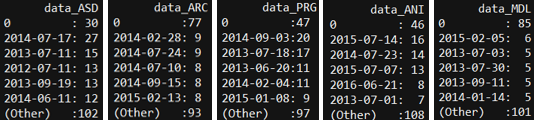
\includegraphics[scale=0.8]{img/sommario_1_anno.png}
                \end{figure}

                Gli esami che non sono stati superati dal maggior numero di istanze dell’intero data set --- e che quindi hanno creato maggiore difficoltà agli studenti --- sono, \footnote{piuttosto comprensibilmente,} Matematica Discreta e Logica e Architetture degli Elaboratori. Si è inoltre notato nella matrice della derivazione standard mostrata in Figura \ref{esami1anno_stddev} che quei due esami presentano una differenza rispetto agli altri. Vale la pena di indagare oltre.

                \begin{figure}
                    \centering
                    \caption{dettaglio sui voti e C.F.U. di Matematica Discreta e Logica}
                    \label{mdl}
                	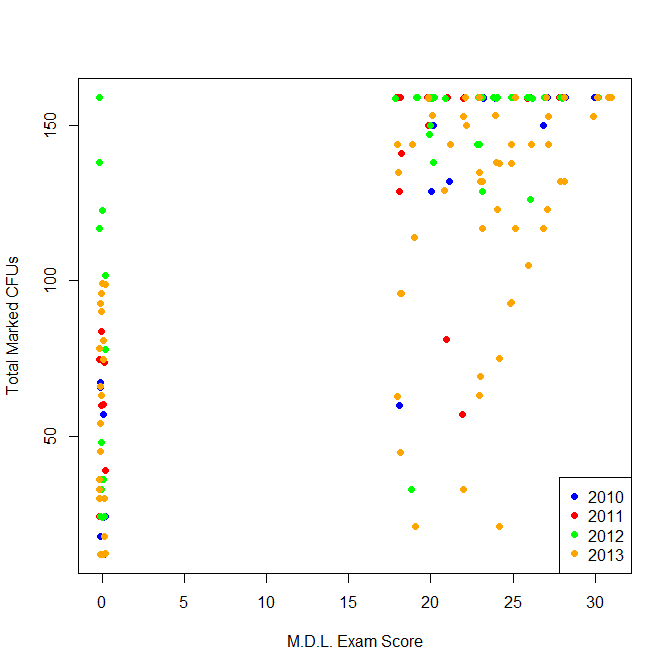
\includegraphics[scale=0.5]{img/scatter_plot_5.png}
                \end{figure}

                \begin{figure}
                    \centering
                    \caption{dettaglio sui risultati di Matematica Discreta e Logica}
                    \label{mdl_2}
                	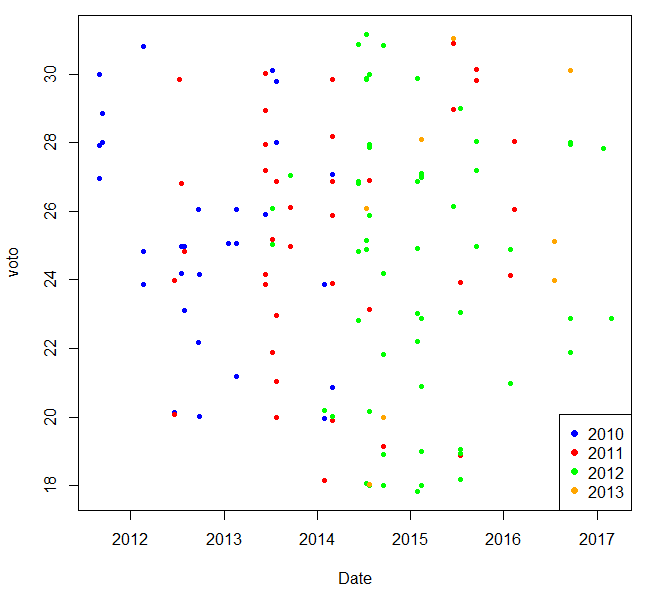
\includegraphics[scale=0.5]{img/scatter_plot_9.png}
                \end{figure}

                \begin{figure}
                    \centering
                    \caption{dettaglio sulla materia Architetture degli Elaboratori}
                    \label{ade}
                	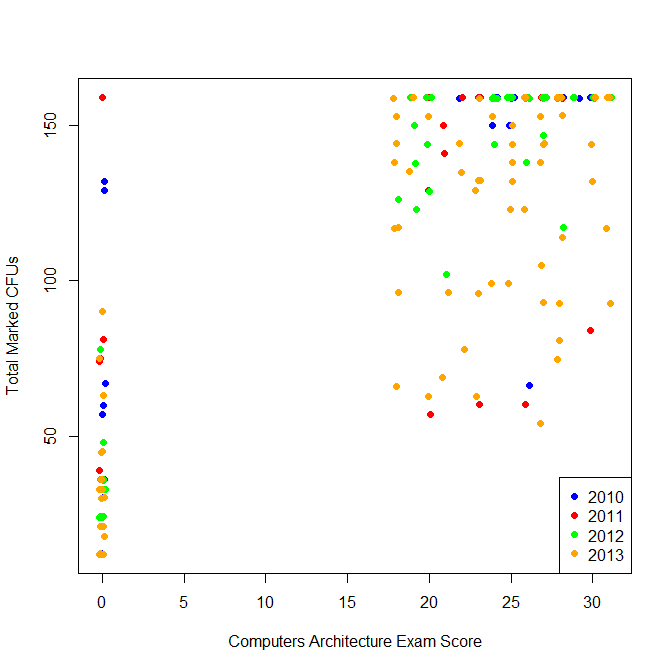
\includegraphics[scale=0.5]{img/scatter_plot_6.png}
                \end{figure}

                Si veda il grafico di dispersione specifico per Matematica Discreta e Logica in Figura \ref{mdl}: si riesce a notare una blanda tendenza dei Credti Formativi Unitari ottenuti in totale dallo studente ad aumentare proporzionalmente al voto ottenuto. C’è inoltre una chiara indicazione che molti studenti –-- con quelli della coorte 2012 a estremizzare questa caratteristica –-- hanno ottenuto comunque molti C.F.U. senza superare questo esame. Inoltre, incrociando il voto conseguito e la data in cui l’esame è stato superato (si veda la Figura \ref{mdl_2}), si riescono a notare due aspetti:

                \begin{itemize}
                    \item chi ha dato l’esame al primo appello del suo anno, ha conseguito un voto alto (si vedano ad esempio gli studenti dell’annata 2010)
                    \item la maggioranza degli studenti ha superato Matematica Discreta e Logica qualche anno dopo il suo anno di immatricolazione (comportamento estremizzato dagli studenti di coorte 2012)
                \end{itemize}

                Nel caso di Architetture degli Elaboratori, della quale possiamo vedere un grafico di dispersione dettagliato in Figura \ref{ade}, le tendenze evidenziate prima sono mitigate. Rimane comunque importante la quantità di studenti che hanno conseguito molti crediti senza superare l’esame: si potrebbe speculare che l’ignorare certi esami sia una pratica comune nel pool di studenti descritti dal data set.

            \subsubsection{Esami su argomenti informatici}

                \begin{figure}
                    \centering
                    \caption{grafico di dispersione relativo agli esami di informatica}
                    \label{esami_inf}
                	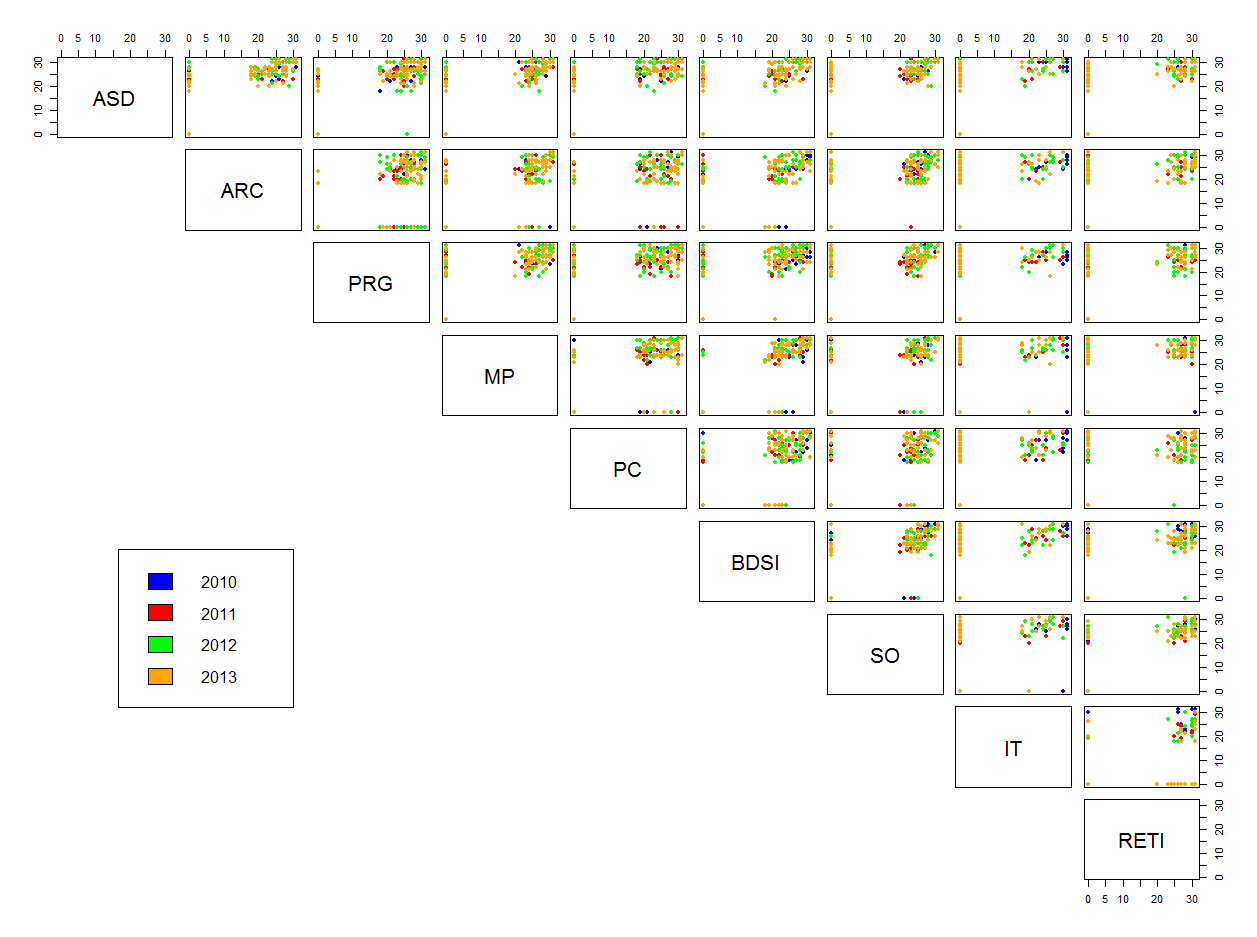
\includegraphics[scale=0.32]{img/scatter_plot_7_gen.png}
                \end{figure}

                \begin{figure}
                    \centering
                    \caption{matrice di correlazione relativa agli esami di informatica}
                    \label{esami_inf_corr}
                	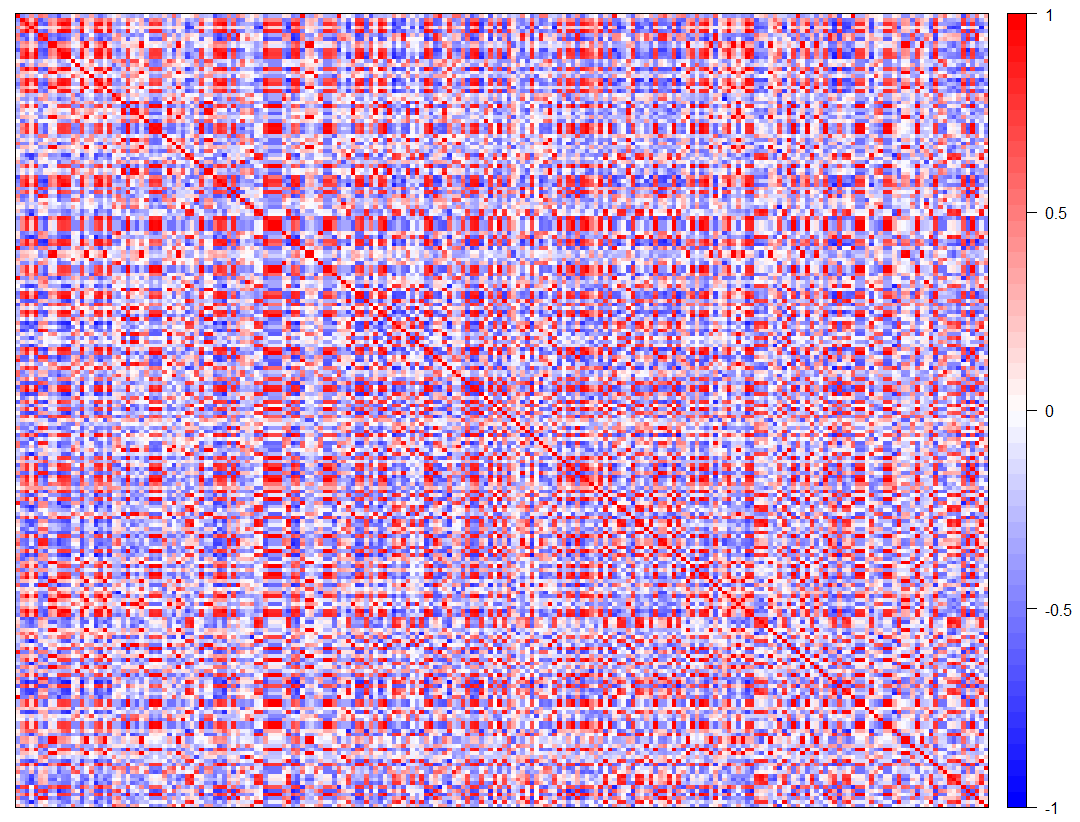
\includegraphics[scale=0.32]{img/corr_matrix_2.png}
                \end{figure}

                \begin{figure}
                    \centering
                    \caption{matrice della deviazione standard relativa agli esami di informatica}
                    \label{esami_inf_stddev}
                	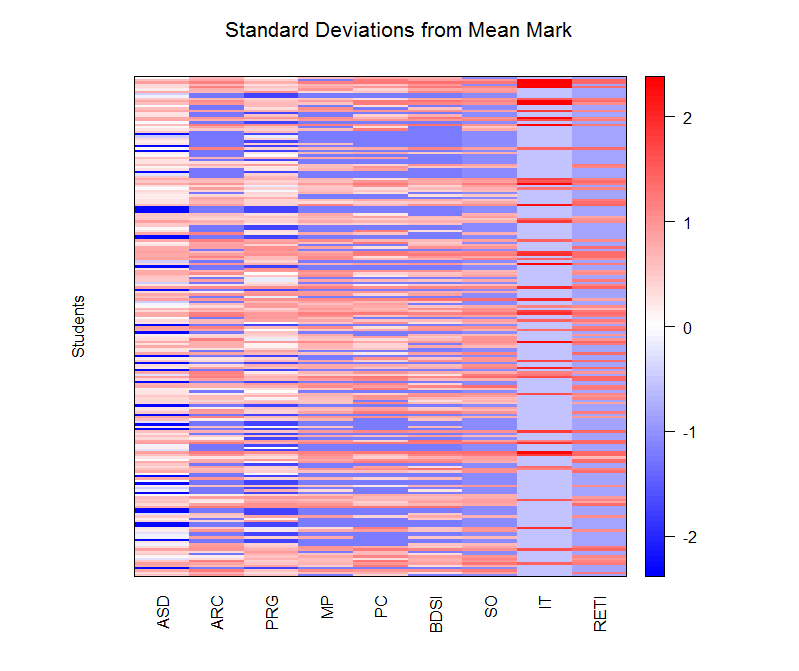
\includegraphics[scale=0.32]{img/std_dev_matrix_2.png}
                \end{figure}

                \begin{figure}
                    \centering
                    \caption{sommario del voto di Informatica Teorica}
                    \label{it}
                	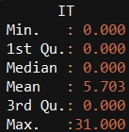
\includegraphics[scale=0.8]{img/it.png}
                \end{figure}

                Riguardo agli esami a contenuto prevalentemente informartico, sono state effettuate analoghe analisi visive. Poco è stato notato dal grafico di dispersione in Figura \ref{esami_inf} e dalla matrice di correlazione in Figura \ref{esami_inf_corr}. Invece, dalla matrice della deviazione standard in Figura \ref{esami_inf_stddev} è stato possibile trarre una interessante deduzione: con l’avvicinarsi agli esami del terzo anno –-- eccezione fatta per Architetture degli Elaboratori –-- si nota che il voto conseguito da ogni studente tende a discostarsi sempre meno dalla media. Nel particolare di Informatica Teorica mostrato in Figura \ref{it}, i pochi studenti che lo superano risultano ampiamente sopra la media. \\

                In ogni caso, non appare interessante proseguire sul'analisi con tecniche di \textit{data mining} su questa suddivisione.

            \subsubsection{Esami su argomenti matematici}

                \begin{figure}
                    \centering
                    \caption{grafico di dispersione relativo agli esami di matematica}
                    \label{esami_mat}
                	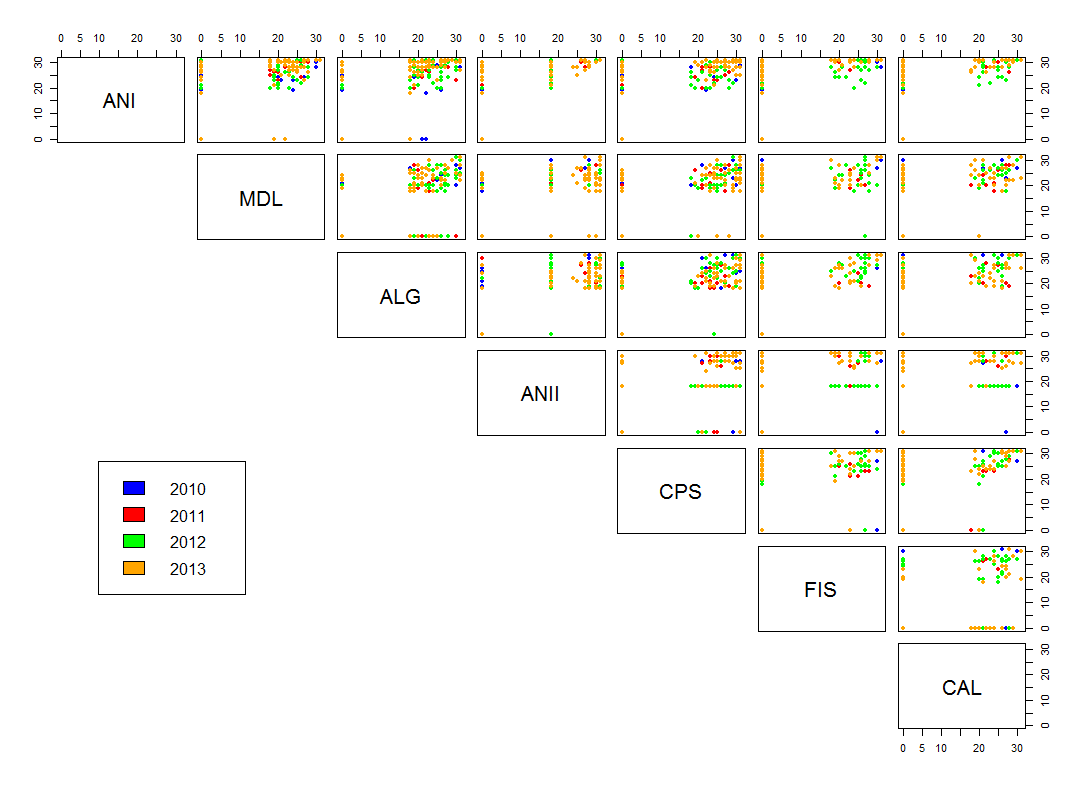
\includegraphics[scale=0.32]{img/scatter_plot_8_gen.png}
                \end{figure}

                \begin{figure}
                    \centering
                    \caption{matrice di correlazione degli esami di matematica}
                    \label{esami_mat_corr}
                	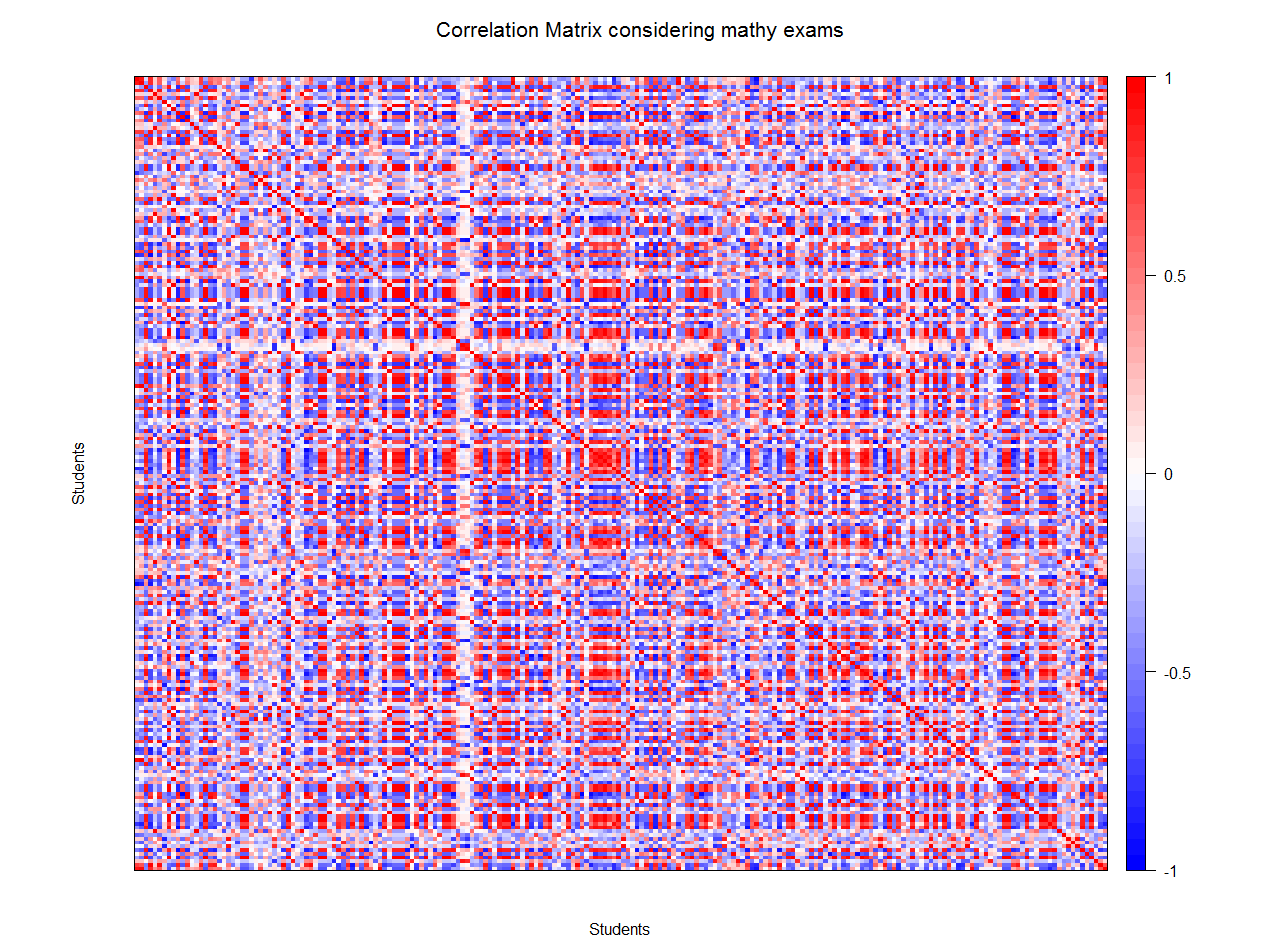
\includegraphics[scale=0.32]{img/corr_matrix_3.png}
                \end{figure}

                \begin{figure}
                    \centering
                    \caption{matrice della deviazione standard relativa agli esami di matematica}
                    \label{esami_mat_stddev}
                	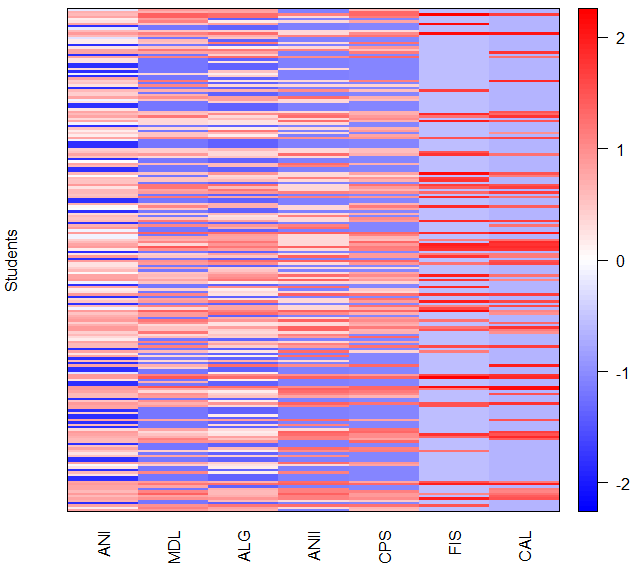
\includegraphics[scale=0.32]{img/std_dev_matrix_3.png}
                \end{figure}

                Riguardo a questa partizione degli esami, di cui si può vedere un grafico di dispersione generale in Figura \ref{esami_mat}, un aspetto che balza immediatamente alla vista è l’enorme quantità di studenti che ha conseguito 18 ad Analisi 2. Data la natura del corso, questa non è affatto un'anomalia, pertanto non appare interessante; inoltre, potrebbe addirittura risultare distorcente rispetto ad una ipotetica \textit{cluster analysys}, perciò occorrerebbe considerarla preventivamente.

                Sulla matrice di correlazione in Figura \ref{esami_mat_corr}, si notano due aspetti interessanti: una fascia di studenti con correlazione nulla e una «casella» di forti correlazioni all’incirca nel centro della matrice. Dei due, il primo è sicuramente il più inusuale. Quale aspetto reale potrebbe generare una osservazione come questa?

                Riguardo alla matrice della deviazione standard in Figura \ref{esami_mat_stddev}, si possono notare le stesse caratteristiche evidenziate per quanto riguarda gli esami a tema principalmente informatico. In questo caso, il ruolo del cattivo non lo interpreta più Informatica Teorica ma è condiviso da Fisica Generale e Calcolo Numerico\footnote{Calcolo Numerico tratta argomenti che trascendono i confini fra l’informatica e la matematica. Si è scelto d'inserirlo in questa partizione, ma è stata una decisione puramente arbitraria.}.

                Analogamente alla suddivisione precedente, anche per questa partizione di esami non appare interessante proseguire l'analisi con tecniche di \textit{data mining}.

        \subsection{Conclusioni}

            Da quello che abbiamo visto, una \textit{cluster analysy} mirata alle prestazioni generali degli studenti potrebbe dare buoni risultati. Inoltre, come si è potuto intuire dal caso di Matematica Discreta e Logica, questo data set racchiude importanti informazioni nelle coppie di valori $(data, voto)$: si potrebbe pensare di estrarre in qualche senso dei \textit{pattern sequenziali} relativi all'ordine in cui vengono superati i vari esami dell'intero Corso di Laurea. \\

            Inoltre, è apparso chiaro anche un altro aspetto: osservare il comportamento dei dati istanza per istanza è stato senza dubbio utile, ma in un data set come questo, in cui gli studenti appartengono a una precisa coorte di immatricolazione, può essere importante catturare gli aspetti fondamentali di ciascuna \textit{classe di record} --- appunto, la coorte di immatricolazione. Si potrebbe quindi pensare di effettuare una massiccia aggregazione di tutti i dati per osservare le differenze fra le classi.

    \section{Data Set: Valutazioni degli Insegnamenti}

        Sebbene questa porzione di dati a disposizione sia quella dalla mole più elevata, si è ritenuto che essa possa esprimere la sua maggiore utilità se impiegata insieme all'altro dataset che abbiamo deciso di considerare principale. Questo comporterà ovviamente la necessità di efettuare una \textbf{join} di qualche tipo fra i due insiemi di dati.\\
        
        Inoltre, si ribadisce che si tratta di dati sì aggregati, ma coprenti comunque un ampio spettro di aspetti di ogni corso. Pertanto, effettuare un'analisi approfondita sullo stile di quella fatta sul data set degli studenti darebbe risultati dispersivi e di difficile interpretazione. \\

        Ci si riserva quindi di adottare un approccio non convenzionale: ritardare l'analisi visiva di questo data set, effettuandola \textbf{dopo} una massiccia aggregazione eseguita nella fase di \textit{preprocessing}. A questo proposito, rimangono valide le considerazioni espresse per il dataset degli studenti riguardo all'osservare il comportamento di ciascuna \textit{classe di record} --- in questo caso, l'Anno Accademico di riferimento.

    \section{Scelta delle Tecniche da Impiegare}

        Come risultato ultimo di questa fase, si è stati in grado di decidere il tipo di tecniche di \textit{preprocessing} e \textit{data mining} che sarà opportuno utilizzare per proseguire lo studio di questi dati. \\

        Si prevede di impiegare queste tecniche:

        \begin{itemize}
            \item \textit{tecniche di visualizzazione} con focus sulle \textit{classi di record} dei due data set;
            \item \textit{cluster analysys} sulle prestazioni generali degli studenti;
            \item individuazione dei \textit{pattern sequenziali frequenti} nell'ordine di superamento degli esami;
            \item \textit{cluster analysys} sulla relazione fra prestazioni degli studenti e valutazioni dei corsi;
            \item ricerca di \textit{regole associative} fra i risultati conseguiti in un dato esame e la valutazione del suo corso.
        \end{itemize}

        Al fine di utilizzarle al meglio, occorre preparare nella fase di \textit{preprocessing} i seguenti data set:

        \begin{itemize}
            \item prestazioni generali degli studenti aggregate per coorte di immatricolazione --- \textit{visualizzazione};
            \item valutazione degli insegnamenti aggregate per Anno Accademico --- \textit{visualizzazione};
            \item join dei due insiemi di dati con attributi continui --- \textit{clustering};
            \item join dei due insiemi di dati con attributi discreti --- \textit{analisi associativa};
            \item sequenze ordinate di esami superati --- \textit{pattern sequenziali}.
        \end{itemize}

        Altre \textit{cluster analysys} sono poi state effettuate direttamente sul dataset della carriera degli studenti con minima preparazione, essendo esso già predisposto all'utilizzo con questo tipo di algoritmi.

\chapter{Preprocessing}
\label{ch:prepr}

Quella che sarà descritta in questo capitolo è sicuramente la fase più impegnativa e delicata dell'intero lavoro. Vista quindi l'importanza che l'attività di \textit{preprocessing} ha rivestito, è stato scelto di descriverla con un elevato livello di dettaglio, evidenziando passaggio per passaggio le operazioni necessarie per dare all'insieme di dati grezzi una forma adeguata al tipo di analisi che ci si è prefissati di fare. \\

Nell'illustrare i vari procedimenti, per favorire una spiegazione lineare e il più possibile comprensibile, si impiegherà ancora la metafora della lavorazione meccanica, intesa in questo caso come una sgrossatura volta ad ottenere un semilavorato --- il data set \textit{preprocessato}, pronto per essere ulteriormente lavorato con le tecniche di \textit{data mining}. Ricordando quanto affermato nell'introduzione della sezioni precedenti, i dati iniziali rappresentano il pezzo grezzo da lavorare, mentre le tecnologie scelte gli utensili da impiegare nella sgrossatura.

\section{Preparazione dell'Ambiente di Lavoro}

	\subsection{Ottenere gli strumenti necessari}

		Innanzitutto è necessario predisporre gli utensili necessari al lavoro da svolgere --- fuor di metafora, si tratta di installare i programmi necessari al \textit{preprocessing}. Come abbiamo detto nella sezione dedicata alla \textit{technology stack}, abbiamo bisogno del \textit{d.b.m.s.} MongoDB e del suo \textit{driver}\footnote{il termine \textit{driver} non è perfettamente proprio per descrivere quella che in realtà è una semplice implementazione in Python delle \textit{A.P.I.} di MongoDB, ma colloquialmente rende bene l'idea della funzione di \texttt{pymongo}.}.

		La piattaforma impiegata è un personal computer con sistema operativo Arch Linux, perciò occorrerà installare MongoDB su di essa. Questo può essere fatto in modo estremamente agile, scaricando i pacchetti \texttt{mongodb} e \texttt{mongodb-tools} dalle repository ufficiali con il seguente comando:

		\begin{lstlisting}[language=bash,caption={installazione di MongoDB}]
			sudo pacman -S mongodb mongodb-tools --noconfirm
		\end{lstlisting}

		\vspace{0.3cm}

		Per ottenere \texttt{pymongo}, invece, occorre utilizzare il \textit{package manager} di Python, \texttt{pip}, invocandolo semplicemente come segue:

		\begin{lstlisting}[language=bash,caption={installazione di pymongo}]
			pip install pymongo
		\end{lstlisting}

		\vspace{0.3cm}

		A questo punto disponiamo degli utensili necessari per la nostra lavorazione.

	\subsection{Inizializzazione di un server MongoDB}

		Predisposti gli utensili, occorre adesso avviare la macchina e montare il pezzo --- in una \textit{vera} lavorazione meccanica, ovviamente \textit{prima} si monta l'utensile e si posiziona il pezzo, \textit{poi} si avvia la macchina; in questo caso, occorre avviare prima un processo di MongoDB affinché si possano importare i dati grezzi in uno \textit{schema} ed organizzarli in \textit{collections}, per poi lavorarli tramite \texttt{pymongo}. \\

	MongoDB fornisce un database estremamente veloce, e di default utilizza come supporto fisico di memorizzazione una cartella sul disco di installazione. La macchina utilizzata dispone di un disco a stato solido come unità di memoria non volatile, perciò le velocità di lettura e scrittura nel database di MongoDB risulterebbero ottime anche nella configurazione standard. Tuttavia, sia per migliorare ulteriormente le performances delle operazioni che per preservare la vita del disco\footnote{le celle di memoria degli SSD, o dischi a stato solido, possono sopportare un numero limitato di scritture prima di rovinarsi.}, è stato scelto di creare un \textit{ramdisk}\footnote{\textit{filesystem} implementato in un'area di RAM; è una tecnica per velocizzare estremamente le operazioni di lettura e scrittura, ma dato che il \textit{filesystem} è implementato su memoria volatile, i dati scritti in esso vengono persi dopo lo spegnimento della macchina.} da far utilizzare a MongoDB. \\

	Per pura comodità, le operazioni necessarie per realizzare quanto appena descritto sono state delegate ad uno script:

	\begin{lstlisting}[language=bash,caption={script di lancio di un server MongoDB}, numbers=left, stepnumber=1]
		#!/bin/zsh
		sudo killall mongod
		yes | rm -rf /mnt/ramdisk/db
		mkdir db /mnt/ramdisk/db
		mongod --dbpath=/mnt/ramdisk/db
	\end{lstlisting}

	\vspace{0.3cm}

	Nella \textit{shell} con cui è stato lanciato, si può vedere lo \textit{standard output} del processo \texttt{mongod}. Significa che MongoDB è attivo ed invocabile tramite gli strumenti a nostra disposizione.

	\subsection{Importazione dei Dati Grezzi}

	A questo punto, sia la macchina che gli utensili sono pronti: occorre posizionare il pezzo grezzo da lavorare, ovvero importare i dati in MongoDB. \\

	Come visto nel capitolo precedente, i dati a disposizione sono contenuti in otto file \texttt{csv}: si manterrà questa struttura --- almeno inizialmente --- importando quindi ogni file in una sua \textit{collection}. Come si può vedere di seguito, questa operazione è stata descritta nel \texttt{makefile} con l'etichetta \texttt{import}:

	\begin{center}
		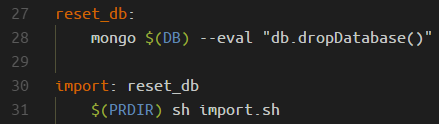
\includegraphics[scale=0.7]{img/import.png}
	\end{center}

	Le variabili \texttt{\$(DB)} e \texttt{\$(PRDIR)} sono specifiche dell'ambiente predisposto\footnote{per un esempio pratico, si consulti l'intero \texttt{makefile} riportato in \ref{appendix:makefile}.}. Essa si può lanciare con il seguente semplice comando di \texttt{shell}:

	\begin{lstlisting}[language=bash,caption={importazione dei dati in MongoDB}]
		make import
	\end{lstlisting}

	\vspace{0.3cm}

	La vera e propria invocazione del comando necessario all'import dei file nel database --- \texttt{mongoimport}, del pacchetto \texttt{mongodb-tools} --- è stata delegata in un file esterno al \texttt{makefile}, per preservare la compattezza e la brevità di quest'ultimo. Si veda comunque di seguito come è struturata la chiamata a \texttt{mongoimport} per uno degli otto file: 

	\begin{lstlisting}[language=bash,caption={dettaglio dell'importazione dei dati in MongoDB}]
		mongoimport -d exams -c rawStudentsPr1013 --type csv --file ../raw/prod_stud_10-11-12-13.csv --headerline
	\end{lstlisting}

	\vspace{0.3cm}

	Il comando, come ogni chiamata da \texttt{shell}, ha degli argomenti che ne specificano il comportamento. In questo caso, sono:

	\begin{itemize}
		\item \texttt{-d}: il database nel quale importare i dati;
		\item \texttt{-c}: la collection nella quale inserire i dati;
		\item \texttt{-type}: il tipo del file da leggere;
		\item \texttt{-file}: il riferimento al file;
		\item \texttt{--headerline}: indica che gli attributi delle istanze sono specificati nella prima riga del file.
	\end{itemize}

	A questo punto, nel database \texttt{exams} di MongoDB ci sono otto \textit{collections}, contenenti i \textit{documenti} che rappresentano le istanze dei dati a disposizione.

\section{Aggregazione per Anno Accademico}

	Avendo predisposto tutto, si può procedere con la prima lavorazione da fare. \\
	
	Si comincia intanto con l'ottenere dei data set \textit{minimali}, uno per le valutazioni dei corsi, l'altro per la produttività degli studenti, condensando in essi le informazioni principali contenute in quello delle prestazioni degli studenti in pochi parametri relativi ad un certo anno accademico. \\

	\subsection{Produttività degli Studenti}

		L'obiettivo è sintetizzare le informazioni sulla produttività degli studenti nei seguenti attributi:

		\begin{itemize}
			\item coorte di immatricolazione;
			\item numero di studenti totali;
			\item percentuale di studenti laureati;
			\item valutazione media ottenuta al test di ingresso;
			\item voto medio ottenuto agli esami;
			\item ritardo medio con cui è stato dato un esame.
		\end{itemize}

		Considerando il tipo dei dati a disposizione, occorrerà innanzitutto aggregare le istanze dei vari studenti in modo opportuno. Questo viene fatto utilizzando un modulo Python programmato \textit{ad hoc}, del quale si riporta di seguito una significativa porzione a titolo di esempio: \\

		\lstinputlisting[language=python,firstline=26,lastline=77, caption={mymodules/aggregs.py}]{../prepr/mymodules/aggregs.py}

		\vspace{0.3cm}

		L'oggetto definito nella porzione di codice appena mostrata viene impiegato per realizzare una prima aggregazione per corsi dei risultati dei singoli studenti. Si può usare questo risultato intermedio per ricavare le informazioni prefissate come necessarie, usando un altro apposito script Python: \\

		\lstinputlisting[language=python, caption={dataset\_stud\_gen.py}]{../prepr/dataset_stud_gen.py}

		\vspace{0.3cm}

		Questo codice produce una \textit{collection} che contiene esattamente il data set che ci si è prefissati di ottenere, calcolando un ritardo 	approssimativo medio (in semestri), la percentuale di studenti che hanno finito il corso di laurea nell'arco temporale a disposizione e le varie medie 	degli altri attributi.\\

		\begin{tabular}{llllll}
		\hline
		Coorte & N. & Laureati {[}\%{]} & Test Ingresso & Voto & Ritardo \\ \hline
		2010 & 30 & 6.67 & 15.4 & 25.5 & 0.81 \\
		2011 & 39 & 10.26 & 13.26 & 24.81 & 1.07 \\
		2012 & 58 & 25.86 & 14.05 & 24.79 & 1.01 \\
		2013 & 80 & 11.25 & 14.39 & 24.98 & 0.77 \\ \hline
		\end{tabular}

		\vspace{0.3cm}

		Il lancio di tutte queste operazioni è descritto nella ricetta \texttt{stud\_gen} del \texttt{makefile}.

	\subsection{Valutazione degli Insegnamenti}

		Analogamente a quanto fatto nella sezione immediatamente precedente, per questa famiglia di dati si vuole ottenere una aggregazione che riassuma i seguenti attributi:

		\begin{itemize}
			\item anno accademico
			\item numero di valutazioni registrate
			\item valutazione complessiva media dei corsi
			\item deviazione standard delle valutazioni
			\item percentuale delle valutazioni sufficienti
		\end{itemize}

		In questo caso è tutto più semplice, in quanto i dati relativi alla valutazione dei corsi sono già in forma aggregata: si tratta quindi solo di comprimerli ulteriormente, facendoli rientrare nello schema che ci si è prefissati. A tale proposito, si utilizzerà ancora il modulo \texttt{aggregs.py}, impiegandone stavolta un oggetto diverso:

		\lstinputlisting[language=python,firstline=172,lastline=259, caption={mymodules/aggregs.py}]{../prepr/mymodules/aggregs.py}

		\vspace{0.3cm}

		Dopo aver usato opportunamente l'oggetto \texttt{ParAggregator}, che mantiene nella \textit{chiave primaria} i corsi, occorre aggregare ancora i dati, rendendo l'Anno Accademico l'unico parametro in grado di discriminare una tupla dall'altra.

		\lstinputlisting[language=python, caption={dataset\_eval\_gen.py}]{../prepr/dataset_eval_gen.py}

		\vspace{0.3cm}

		Il lancio combinato di queste porzioni di codice, specificato con la ricetta \texttt{teval\_gen} del \texttt{makefile}, produce un data set di questo tipo:\\

		\begin{tabular}{lllll}
		\hline
		A. A. & Val. Media & Std. Dev. Val. & Val. Sufficienti {[}\%{]} & N. \\ \hline
		2010-2011 & 7.54 & 1.74 & 82.14 & 17 \\
		2011-2012 & 7.93 & 1.61 & 90.68 & 26 \\
		2012-2013 & 7.98 & 1.7 & 90.55 & 30 \\
		... & ... & ... & ... & .. \\ \hline
		\end{tabular}

		\vspace{0.3cm}

\section{Join dei due insiemi di dati}

	Il \textit{join} delle due famiglie di dati è l'operazione più delicata fra quelle di tutto il \textit{preprocessing}. Occorre definire bene gli attributi sui quali definire la relazione, e prestare in generale attenzione ai vari errori che, se commessi, comprometterebbero totalmente il significato del risultato. \\

	\subsection{Join con valutazioni estese e attributi continui}

		Per prima cosa, si è realizzata una \textit{join} fra i due data set aggregando i dati degli studenti \textbf{per esame}, e i dati delle valutazioni dei corsi \textbf{per paragrafo}. Osservando l'albero delle dipendenze specificato nel \texttt{makefile} riportato in \ref{appendix:makefile}, si può notare che sono state prima realizzate le aggregazioni dei singoli data set e, solo successivamente, performata l'operazione di \textit{join} fra di essi. \\

		L'aggregazione dei dati degli studenti avviene in modo del tutto analogo a quanto fatto nella sezione precedente con l'oggetto \texttt{StudAggregator} del modulo Python \texttt{aggregs.py}. \\

		Per quanto riguarda l'aggregazione dei dati delle valutazioni dei corsi, sono state effettuati vari passaggi per arrivare ad aggregare ... descritti in \ref{appendix:teval}. \\

		Predisposti opportunamente i due insiemi di dati in due \textit{collection}, la fase di merge è stata portata avanti grazie all'ausilio di un altro modulo Python scritto \textit{ad hoc}: si tratta dell'oggetto \texttt{Merger}, contenuto nel file \texttt{merge.py}, il cui codice è riportato qui sotto:

		\lstinputlisting[language=python, caption={mymodules/merge.py}]{../prepr/mymodules/merge.py}

		Tale oggetto viene utilizzato nello script \texttt{dataset\_merge.py}. Il \textit{join} avviene, chiaramente, sugli attributi \textbf{Anno Accademico} e \textbf{Corso d'Esame}, trasferendo gli attributi specifici di una collezione direttamente nell'altra in questo modo:

		\lstinputlisting[language=python, caption={dataset\_merge.py}]{../prepr/dataset_merge.py}

		A questo punto, la collezione risultante da queste operazioni ha le caratteristiche cercate. Tuttavia, presenta delle "sbavature" che è conveniente rimuovere prima di impiegarla efficacemente nel \textit{data mining}. Per eliminarle, ci si avvale di un ulteriore modulo Python realizzato per l'occasione, \texttt{cleanings.py}, il cui codice viene omesso in questa sezione per ragioni di brevità\footnote{Tale codice è comunque riportato in \ref{appendix:clean}}. \\

		Tutte queste operazioni sono invocate tramite le seguenti ricette, definite nel \texttt{makefile}:
		
		\begin{center}
			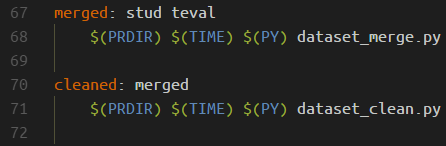
\includegraphics[scale=0.7]{img/join.png}
		\end{center}

		Concluso quanto appena descritto, si è creato un primo data set utilizzabile. Esso presenta i seguenti attributi, tutti di tipo	\textit{continuo} --- tranne ovviamente le \textit{chiavi primarie} e le istanze considerate per la produttività degli studenti:

		\begin{itemize}
			\item Anno Accademico
			\item Hash Docente/i
			\item Insegnamento
			\item \textbf{Produttività Studenti}:
				\subitem N [istanze]
				\subitem Ritardo >=1sem [percent]
				\subitem Ritardo [semestre, media]
				\subitem Voto >= 24 [perc]
				\subitem Voto [media]
				\subitem Voto [std dev]
			\item \textbf{Valutazione degli Aspetti Specifici del Corsi di Studi}:
				\subitem N [istanze]
				\subitem Std Dev [media pesata]
				\subitem Val >= 6 [percent]
				\subitem Val [media pesata]
			\item \textbf{Valutazione dell'adeguatezza delle Aule e delle Attrezzature}:
				\subitem \textit{attributi identici alla valutazione precedente}
			\item \textbf{Valutazione sul Docente}:
				\subitem \textit{attributi identici alla valutazione precedente}
			\item \textbf{Valutazione sulla Disponibilità di Informazioni Aggiuntive}:
				\subitem \textit{attributi identici alla valutazione precedente}
			\item \textbf{Valutazione dell'Organizzazione del Corso di Studi}:
				\subitem \textit{attributi identici alla valutazione precedente}
			\item \textbf{Valutazione dell'Organizzazione della Didattica}:
				\subitem \textit{attributi identici alla valutazione precedente}
			\item \textbf{Soddisfazione degli Studenti riguardo al Corso di Studi}:
				\subitem \textit{attributi identici alla valutazione precedente}
		\end{itemize}

		Come si può notare agilmente, il data set presenta un gran numero di attributi, molti fin troppo specifici per poterne estrarre un qualche tipo di informazione generale. Pertanto, è stato deciso aggregare ulteriormente fra loro gli attributi relativi alle valutazioni dei corsi, per sfoltire significativamente la quantità di campi presenti.
		
	\subsection{Join con valutazioni aggregate e attributi continui}
	
	\subsection{Attributi discreti}

\section{Sequenze ordinate di esami superati}

\section{Estrazione dei data set preprocessati}

	\begin{center}
		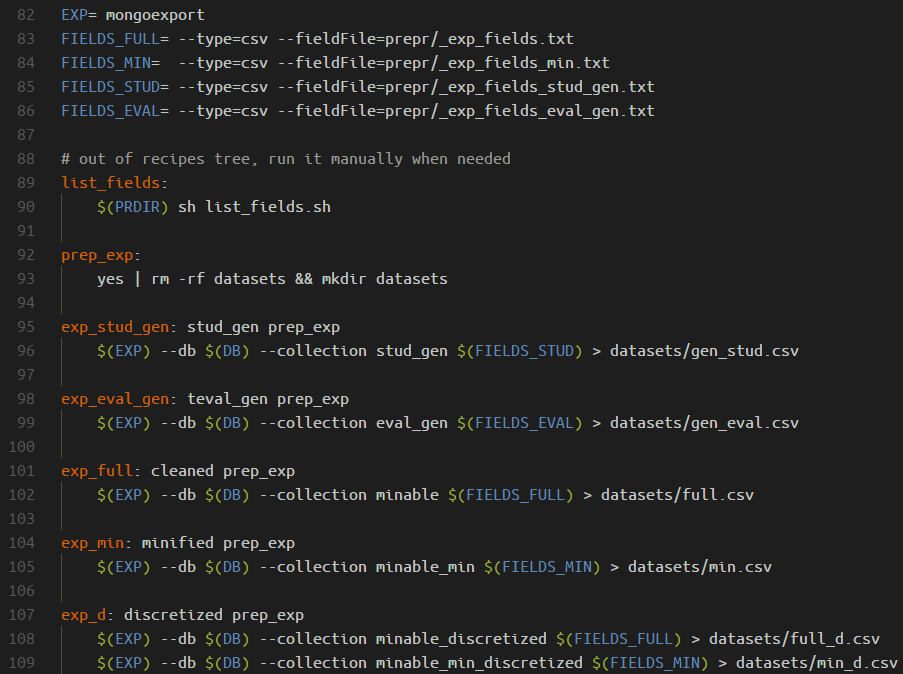
\includegraphics[scale=0.7]{img/export.png}
	\end{center}

	\lstinputlisting[language=bash,caption={script di shell per ottenere una lista degli attributi dei documenti in una collezione}, numbers=left, stepnumber=1]{../prepr/list_fields.sh}

	\lstdefinelanguage{JavaScript}{
  		keywords={break, case, catch, continue, debugger, default, delete, do, else, finally, for, function, if, in, instanceof, new, return, switch, this, throw, try, typeof, var, void, while, with},
 		morecomment=[l]{//},
  		morecomment=[s]{/*}{*/},
  		morestring=[b]',
  		morestring=[b]",
  		sensitive=true
	}

	\lstinputlisting[language=JavaScript,caption={script della shell di MongoDB per ottenere la lista degli attributi dei documenti in una collezione}, numbers=left, stepnumber=1]{../prepr/list_attr.mongosh}

\chapter{Data Understanding per Classi}
\label{ch:visual}

In questo capitolo si andranno a impiegare i due data set minimali, ottenuti mediante una massiccia aggregazione dei dati a disposizione effettuata nella precedente fase di \textit{preprocessing}, come base per l'utilizzo di alcune tecniche di visualizzazione. \\

Il fine è quello di evidenziare elementi che facciano intuire un \textit{trend} fra le varie \textbf{classi di record} in cui si è aggregato tutti i dati a disposizione: si sta parlando, ovviamente, delle \textit{coorti di immatricolazione} per quanto riguarda il data set degli studenti, e degli \textit{Anni Accademici} riguardo alle valutazioni dei corsi.

\section{Valutazione dei Corsi}

Per la valutazione dei corsi, si lavorerà sul dataset ottenuto come descritto nella Sezione \ref{prepr:eval_min}. Data la sua dimensione molto ristretta, è possibile riportarlo qui sotto per intero:

\noindent\begin{table}[]
\begin{tabular}{lllll}
\hline
A. A. & N. & Valutazione [1-10] & Std. Dev. Val. & Val. Sufficienti {[}\%{]} \\
& & \textit{media} & \textit{media} & \\
\hline
2010-2011 &  17 & 7.54 & 1.74 & 82.14 \\
2011-2012 &  26 & 7.93 & 1.61 & 90.68 \\
2012-2013 & 30  & 7.98 & 1.7 & 90.55 \\
2013-2014 & 47  & 7.7 & 1.77 & 87.17 \\
2014-2015 &  51 & 7.94 & 1.77 & 89.36 \\
2015-2016 &  49 & 8.01 & 1.76 & 89.94 \\
2016-2017 &  53 & 8.01 & 1.82 & 89.34 \\ \hline
\end{tabular}
\end{table}

    \subsection{Panoramica Generale sulle Valutazioni dei Corsi}
    \label{visual:eval_gen}

    Per inquadrare subito la situazione e mettere a fuoco con un singolo colpo d'occhio le caratteristiche di ogni Anno Accademico, è stato realizzato l'istogramma mostrato in Figura \ref{eval_gen}. \\

    Come si può facilmente verificare con una rapida osservazione del grafico, l'unico attributo che varia sensibilmente è il numero medio di valutazioni dei corsi registrate; si può notare inoltre che esso presenta una tendenza a crescere con l'avanzare dell'Anno Accademico. Per quanto riguarda gli altri attributi, rimangono sostanzialmente simili, fatta eccezione per la percentuale di valutazioni sufficienti registrata negli Anni Accademici 2010-2011, leggermente inferiori rispetto agli altri. \\

    \begin{figure}
        \centering
        \caption{istogramma mostrante una panoramica generale su tutti gli attributi del dataset descritto in Sezione \ref{prepr:eval_min}}
        \label{eval_gen}
        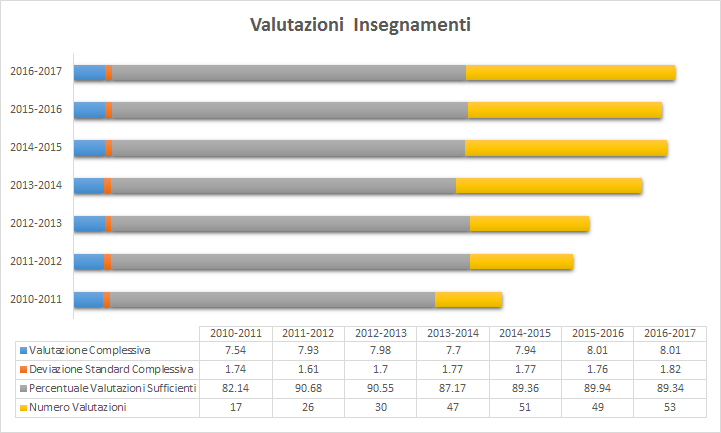
\includegraphics[scale=0.55]{../visual/eval_3.png}
    \end{figure}

    \subsection{Dettaglio sulla Percentuale di Valutazioni Sufficienti}

    Volendo vedere con un maggior livello di dettaglio l'andamento di quest'ultimo aspetto, è stato realizzato un grafico mostrante le percentuali di valutazioni dei corsi sufficienti come serie storica attraverso tutti gli Anni Accademici per i quali si hanno a disposizione delle informazioni. Tale grafico, mostrato in Figura \ref{eval_p}, mostra con maggiore chiarezza quanto si è osservato sull'istogramma generale di Figura \ref{eval_gen}. \\

    \begin{figure}
        \centering
        \caption{serie storica dell'attributo "percentuale di valutazioni sufficienti" attraverso gli Anni Accademici coperti dal data set delle valutazioni dei corsi}
        \label{eval_p}
        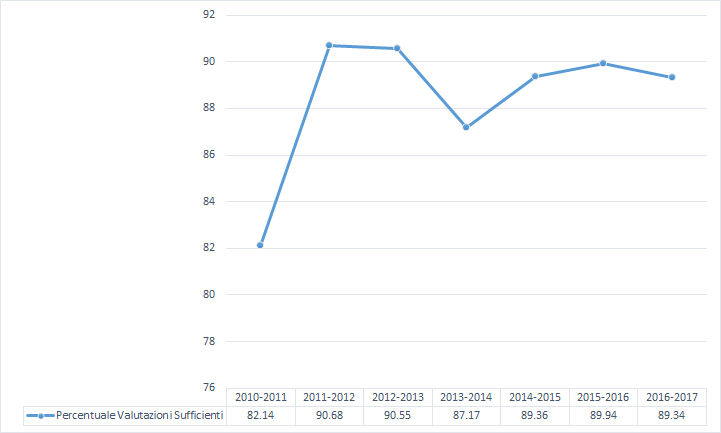
\includegraphics[scale=0.56]{../visual/eval_2.png}
    \end{figure}

\section{Produttività degli Studenti}

    Riguardo ai dati relativi alla produttività degli studenti, il dataset su cui si è lavorato è quello descritto nella Sezione \ref{prepr:stud_min}. Esso è già stato riportato nella sua interezza in tale sede ma, data la sua piccola dimensione, è comunque ripetuto qui di seguito per comodità di consultazione. \\

    \noindent\begin{tabular}{llllll}
		\hline
		Coorte & N. & Laureati {[}\%{]} & Test Ingr. [0-25] & Voto [18-31] & Ritardo [sem.] \\
		 &  & & \textit{media} & \textit{media} & \textit{media}\\
		\hline
		2010 & 30 & 6.67 & 15.4 & 25.5 & 0.81 \\
		2011 & 39 & 10.26 & 13.26 & 24.81 & 1.07 \\
		2012 & 58 & 25.86 & 14.05 & 24.79 & 1.01 \\
		2013 & 80 & 11.25 & 14.39 & 24.98 & 0.77 \\ \hline
	\end{tabular}

    \subsection{Panoramica generale sulla Produttività degli Studenti}

    Per quanto riguarda una preliminare analisi generale dell'intero data set, restano valide le considerazioni espresse in Sezione \ref{visual:eval_gen}. Pertanto, è stato generato un istogramma del tutto analogo a quanto fatto in tale sezione, mostrato in Figura \ref{stud_gen}. \\

    In seguito a un'analisi visiva del grafico, si può notare come gli attributi che più variano sono il numero di studenti imatricolati e la percentuale di studenti laureati entro la fine del periodo in esame. L'andamento degli studenti immatricolati è considerevolmente simile a quello riscontrato sul numero di valutazioni dei corsi registrate, quindi è plausibile supporre una certa correlazione diretta fra i due attributi --- piuttosto banalmente, se ci sono più studenti iscritti, perverranno anche più valutazioni dei corsi.

    \begin{figure}
        \centering
        \caption{istogramma mostrante una panoramica generale su tutti gli attributi generali del dataset descritto in Sezione \ref{prepr:stud_min}}
        \label{stud_gen}
        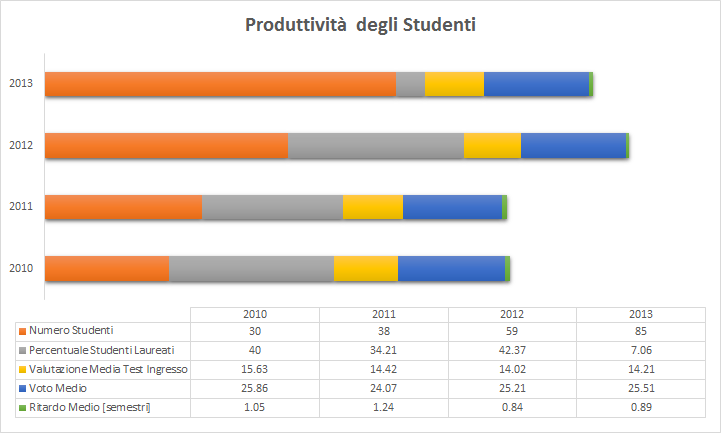
\includegraphics[scale=0.50]{../visual/stud_1.png}
    \end{figure}

    \subsection{Relazione fra Test di Ingresso, Voto Medio e Ritardo}

    Un aspetto curioso sul quale si è voluto fare luce è l'esistenza o meno di una qualche correlazione fra il risultato conseguito nel test di ingresso e le valutazioni ottenute nei successivi esami di profitto. Avendo a disposizione in questa sede entrambi gli attributi in forma aggregata, è stato realizzato il grafico di Figura \ref{test}. \\

    Si noti che gli attributi considerati non esprimono valori nella stessa scala: il test di ingresso prevede un punteggio massimo di 25, mentre per gli esami di profitto il punteggio massimo previsto è di 31 punti\footnote{I voti negli esami vanno ovviamente da 18 a 30, con il 31 a rappresentare in realtà il 30 con lode.}. C'è stato perciò bisogno di effettuare una \textit{normalizzazione} di tali attributi, per poterli confrontare direttamente. \\

    \begin{figure}
        \centering
        \caption{serie temporale mostrante i valori degli attributi normalizzati "voto medio" e "valutazione media al test di ingresso"}
        \label{test}
        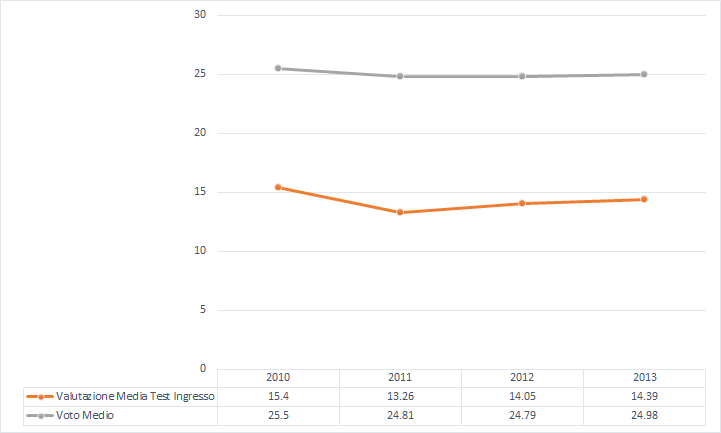
\includegraphics[scale=0.55]{../visual/stud_2.png}
    \end{figure}

    Come si può vedere, pare esserci una correlazione estremamente blanda, ma non risulta così significativa da essere presa in considerazione per ulteriori approfondimenti. Inoltre, si può notare un \textit{offset} abbastanza pronunciato fra i due attributi; concedendoci una speculazione, potrebbe essere dato da un minor impegno degli studenti nel test di ingresso dato dalla sua soglia di sufficienza molto bassa --- 12 punti su 25 --- e dal fatto che il risultato in tale test non impatta in alcun modo la futura carriera accademica. \\

    \begin{figure}
        \centering
        \caption{serie temporale mostrante l'andamento dell'attributo "ritardo medio" relativo al superamento degli esami di profitto}
        \label{ritardo}
        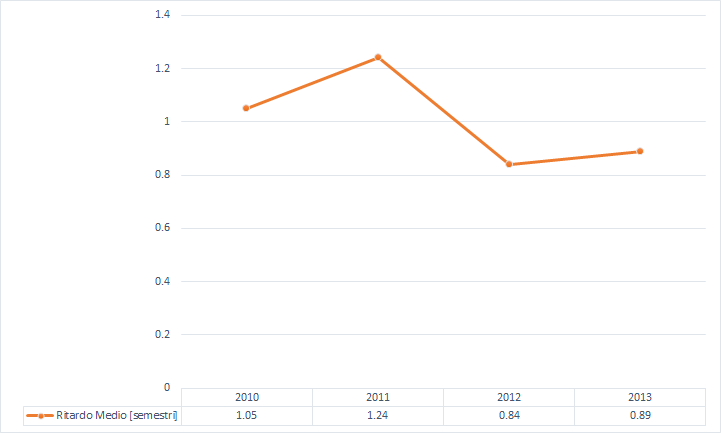
\includegraphics[scale=0.55]{../visual/stud_3.png}
    \end{figure}

    La curiosa flessione della valutazione al test di ingresso fra la coorte di studenti immatricolati nel 2011 trova un riscontro nell'andamento del ritardo medio con cui sono stati superati gli esami di profitto rispetto al loro primo appello, come si può vedere dalla Figura \ref{ritardo}. Comunque, si tratta di una correlazione abbastanza debole, pertanto è stato scelto di limitarsi a notarla, senza proseguire nell'analisi. \\

    \subsection{Percentuale di Studenti Laureati}

    Un indice interessante dell performances di una certa coorte di immatricolazione è la percentuale di studenti che ha terminato con successo il corso di studi entro il periodo di tre anni considerato dai dati a disposizione. Si è quindi deciso di porre attenzione su questo attributo, mostrandolo come serie temporale in Figura \ref{laureati}. \\

    \begin{figure}
        \centering
        \caption{serie temporale mostrante l'andamento dell'attributo "percentuale di studenti laureati entro tre Anni Accademici dall'immatricolazione"}
        \label{laureati}
        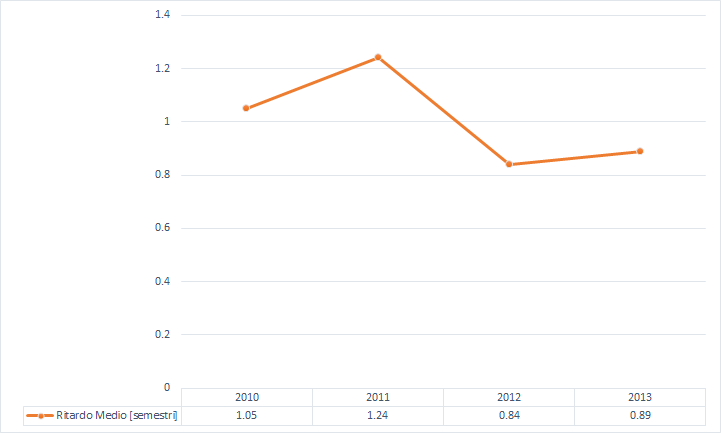
\includegraphics[scale=0.55]{../visual/stud_3.png}
    \end{figure}

    Si nota una sensibile oscillazione di questo valore, che tocca il suo picco massimo nella coorte di studenti immatricolati nel 2012, ma non si è riscontrato --- almeno in seguito a una preliminare analisi visiva --- alcuna correlazione con altri aspetti evidenziati da altri attributi.

\chapter{Cluster Analysys}
\label{ch:cluster}

    In questo capitolo si descriveranno le attività svolte per realizzare dei \textit{clustering} sulle versioni ad attributi continui dei data set prodotti nella fase di \textit{preprocessing} (descritta nel Capitolo \ref{ch:prepr}).

\section{Introduzione alla Cluster Analysys}

    Volendo spendere poche parole per delineare un quadro generale e impiegando una massiccia astrazione dai dettagli, possiamo descrivere un \textit{clustering} come segue, citando direttamente da \cite{clustering}:\\

    "Il \textbf{clustering} o \textbf{analisi dei gruppi} (dal termine inglese \textit{cluster analysis} introdotto da Robert Tryon nel 1939) è un insieme di tecniche di analisi multivariata dei dati volte alla selezione e raggruppamento di elementi omogenei in un insieme di dati."\\

    Volendo sintetizzare ulteriormente questi concetti, si può dire che un \textit{clustering} su di un certo data set è un raggruppamento di istanze \textbf{simili fra loro}. Citando sempre da \cite{clustering}:\\

    "Le tecniche di clustering si basano su misure relative alla somiglianza tra gli elementi. In molti approcci questa similarità, o meglio, dissimilarità, è concepita in termini di distanza in uno spazio multidimensionale. La bontà delle analisi ottenute dagli algoritmi di clustering dipende molto dalla scelta della metrica, e quindi da come è calcolata la distanza. Gli algoritmi di clustering raggruppano gli elementi sulla base della loro distanza reciproca, e quindi l'appartenenza o meno ad un insieme dipende da quanto l'elemento preso in esame è distante dall'insieme stesso."\\

    Questa breve ma efficace descrizione sommaria fornisce già una sufficiente infarinatura riguardo al tipo di azioni da compiere per ottenere un \textit{clustering}: si tratta infatti di cercare all'interno dei data set in esame dei gruppi di istanze simili fra di loro per qualche criterio --- che vedremo essere delle metriche di distanza in uno spazio multidimensionale definito dagli attributi dei dati.\\

    Quanto scritto può essere sufficiente per delineare il quadro generale nel quale si è operato per compiere i passi descritti successivamente. Ovviamente, una trattazione esaustiva sull'argomento necessiterebbe ben altro spazio di quello che si può dedicare in questa tesi di laurea, perciò si rimanda alla consultazione di \cite{dispense} per ulteriori dettagli, qualora quanto sopra riportato non dovesse essere sufficiente per la comprensione di quanto seguirà.

\section{Algoritmi di Clustering}

    La realizzazione di un \textit{clustering} su dei \textit{big data} è ovviamente una di quelle attività che hanno bisogno di essere delegate a un algoritmo per essere eseguite. Si descriveranno in questa sezione alcuni dei più efficaci algoritmi di \textit{clustering} e le implementazioni di Weka.

    \subsection{Algoritmo K-Means}

        Uno dei più noti algoritmi di \textit{clustering} che consente di imporre a priori il numero di \textit{cluster} cercati è senza dubbio \textbf{K-Means}. Come si può leggere in \cite{dispense}:\\

        "The K-means clustering technique is simple [...]. We first choose \textit{K} initial centroids, where \textit{K} is a user-specified parameter, namely, the number of clusters desired. Each point is then assigned to the closest centroid, and each collection of points assigned to a centroid is a cluster. The centroid of each cluster is then updated based on the points assigned to the cluster. We repeat the assignment and update steps until no point changes clusters, or equivalently, until the centroids remain the same." \\

        Il che significa, traducendo e parafrasando:\\

        "La tecnica K-Means è semplice: scegliamo inizialmente \textit{K} centroidi iniziali, dove \textit{K} è il numero di cluster desiderati. Ogni punto del data set è assegnato al centroide più vicino, e ogni collezione di punti assegnati a un centrode è un cluster. Il centroide di ogni cluster viene poi ricalcolato, basandosi sui punti che gli sono stati assegnati. Si ripetono questi passi fino a che nessun punto cambia cluster, o i centroidi non cambiano."\\

        Quindi, si tratta di una procedura iterativa che, a partire da un numero fissato di punti iniziali, chiamati centroidi, migliora ad ogni passo gli assegnamenti fino a che non si raggiunge una situazione di stabilità. \\

        Le librerie di Weka mettono a disposizione una implementazione di K-Means, che permette di configurare un gran numero di parametri (come si può vedere in Figura \ref{kmeans_weka}).

        \begin{figure}
            \centering
            \caption{finestra che mostra i parametri impostabili dell'algoritmo K-Means}
            \label{kmeans_weka}
            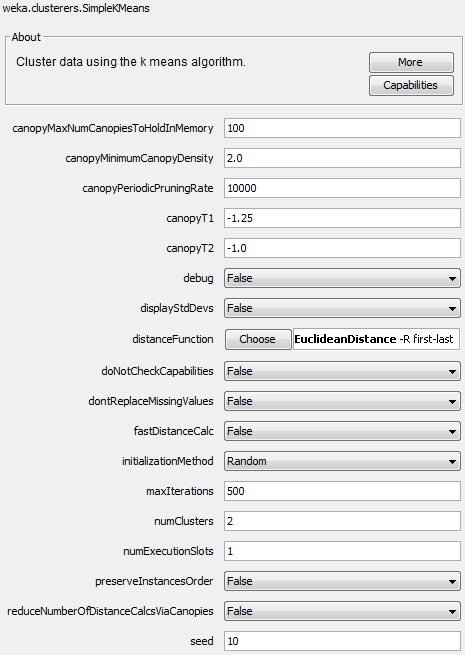
\includegraphics[scale=0.90]{img/cluster_k_means.png}
        \end{figure}

    \subsection{Algoritmo DBSCAN}

        Una algoritmo sostanzialmente diverso dal precedente è DBSCAN, che non si basa sul minimizzare le distanze dal centroide del \textit{cluster}, ma bensì sul raggruppare le istanze del data set in base alla loro \textbf{densità}. \\

        Una informale ma potente descrizione di questo si può leggere in \cite{dispense}:

        "Density-based clustering locates regions of high density that are separated from one another by regions of low density. DBSCAN is a simple and effective density-based clustering algorithm [...]"\\

        Che tradotto significa:\\

        "Le teniche di clustering basate sulla densità individuano regioni dense separate le une dalle altre da regioni meno dense. DBSCAN è un algoritmo di clustering basato sulla densità semplice ed efficace."\\

        Quindi, si può dire che DBSCAN sia un algoritmo che, a differenza di K-Means, non cerca di individuare a quale dei cluster decisi inizialmente appartenga una data istanza, ma individua invece i cluster "naturali" del data set basandosi sulla densità di istanze nelle varie regioni dello spazio multidimensionali definito dagli attributi. \\

        L'implementazione di DBSCAN fornita da Weka, come si può vedere in Figura \ref{dbscan_weka}, è molto basilare, ma totalmente funzionale.

        \begin{figure}
            \centering
            \caption{finestra che mostra i parametri impostabili dell'implementazione di DBSCAN su Weka}
            \label{dbscan_weka}
            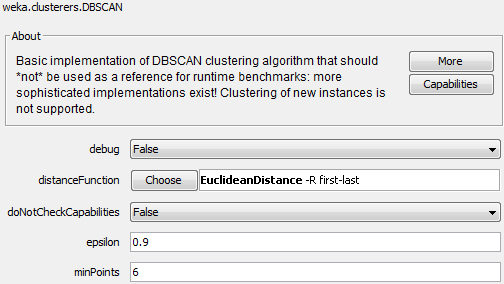
\includegraphics[scale=0.70]{img/dbscan_weka.png}
        \end{figure}

\section{Clustering sulle Valutazioni dei Corsi}

    Una prima serie di tentativi di \textit{cluster analysis} è stata fatta sul data set condensato delle valutazioni dei corsi, utilizzando l'algoritmo K-Means. \\

    Si è ben coscienti che una analisi di questo tipo su un data set che contiene solo sette elementi \textit{generalmente} non avrebbe molto senso, ma in questo caso si può considerare come un approfondimento della fase di \textit{data understanding} su questo data set.

    \subsection{Lancio di K-Means}

        Adottando un metodo empirico di \textit{trial-and-error}, sono state effettuati innumerevoli lanci di K-Means variando di volta in volta i parametri di input. \\

        Quella che segue è la configurazione che genera il miglior risultato ottenuto:

        \begin{center}
            \texttt{weka.clusterers.SimpleKMeans -init 0 -max-candidates 100 -periodic-pruning 10000 -min-density 2.0 -t1 -1.25 -t2 -1.0 -V -M -N 2 -A "weka.core.EuclideanDistance -R first-last" -I 5000 -num-slots 1 -S 997}
        \end{center}

        Nonostante l'elevato numero di parametri a disposizione, in realtà soltanto alcuni hanno influenzato il risultato finale:

        \begin{itemize}
            \item come metrica è stata scelta la \textbf{distanza Euclidea}\footnote{Si tratta di una metrica che misurala distanza fra due punti di uno spazio multidimensionale come la lunghezza del segmento che li unisce.};
            \item sono stati imposti due centroidi iniziali scelti casualmente, ottenendo pertanto un partizionamento con due cluster
        \end{itemize}

        Ai fini del clustering, sono stati considerati soltanto tre attributi: la valutazione complessiva del corso, la deviazione standard delle valutazioni e la percentuali di valutazioni sufficienti.

        \lstinputlisting[caption={Output della console di Weka relativo al lancio di K-Means sul data set delle valutazioni dei corsi}]{../cluster/eval_kmeans.txt}

        \begin{figure}
            \centering
            \caption{sezione dello spazio di esistenza del data set delle valutazione dei corsi lungo il piano definito da "valutazione complessiva" e "percentuale di valutazioni sufficienti", con evidenziato per ogni istanza il cluster di appartenenza}
            \label{eval_kmeans}
            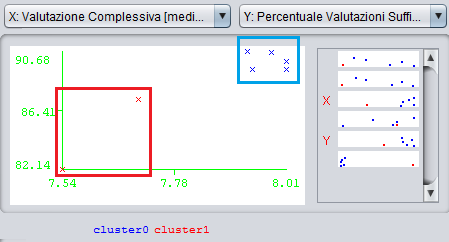
\includegraphics[scale=1.2]{../cluster/eval_kmeans.png}
        \end{figure}

        Come si può vedere dalla Figura \ref{eval_kmeans}, il data set è stato diviso in due cluster che appaiono visivamente ben separati.

        \begin{itemize}
            \item \textbf{Cluster 1} (rosso): A. A. 2013-2014 e 2010-2011
            \item \textbf{Cluster $0$} (blu): gli altri cinque A. A.
        \end{itemize}

\section{Clustering sulla join dei due data set}

    Quanto segue è la parte fondamentale di questa \textit{cluster analysis}, ovvero lo studio della versione ad attributi continui dell'unione dei due data set iniziali.

    \subsection{Lancio di K-Means}

        In modo del tutto analogo a quanto fatto per la precedente attività di clustering, sono state fatte molte prove al fine di raggiungere una configurazione di lancio di K-Means soddisfacente: \\

        \lstinputlisting[caption={Output della console di Weka relativo al lancio di K-Means sul data set risultante dal join delle due collezioni di dati a disposizione}]{../cluster/min_kmeans_2cl.txt}

        Occorre notare varie cose, al fine di comprendere il signficato di quanto è stato ottenuto:

        \begin{itemize}
            \item la \textbf{somma dell'errore quadratico}\footnote{Si tratta di una metrica che da una misura di quanto i punti che compongono il cluster siano distanti dal centroide --- in parole estremamente semplici: più è alto, più il cluster è composto da punti sparsi.} all'interno dei cluster è molto maggiore di quella ottenuta nell'occasione precedente, ma non si può assolutamente fare un confronto diretto fra le due quantità, sia per la diversa natura dell'indagine che per il diverso numero di istanze tenute in considerazione;
            \item al fine di semplificare il significato geometrico della metrica di distanza scelta (quella Euclidea), sono stati presi in considerazione ai fini del clustering soltanto gli attributi più caratterizzanti del dataset:
                \subitem --- Voto medio degli studenti
                \subitem --- Ritardo medio degli studenti
                \subitem --- Valutazione media del corso
            \item sono stati cercati, anche in questo caso, due soli cluster; semanticamente, si può intendere di voler dividere i corsi "migliori", in cui gli studenti hanno prodotto delle buone performance e che la cui didattica ha ricevuto delle buone valutazioni, da quelli "peggiori".
        \end{itemize}

    \subsection{Analisi dei risultati di K-Means}

        Il risultato ottenuto è parzialmente in linea con l'intento che ci si era prefissati. Il cluster identificato da Weka come \textbf{Cluster $0$}, e colorato di \textbf{blu} nei grafici che verranno mostrati, può essere considerato quello dei corsi migliori. Conseguentemente, il \textit{cluster 1} può essere letto come quello dei corsi peggiori rispetto agli altri e rispetto alle metriche considerate. \\

        Si vada innanzitutto a vedere come sono state raggruppate le istanze del data set nei due cluster, rispetto ai tre attributi caratterizzati (Figure \ref{1}, \ref{2} e \ref{3}). Come si può agilmente notare, la divisione che ci si aspettava di vedere è presente.\\

        \begin{figure}
            \centering
            \caption{sezione dello spazio di esistenza del data set delle valutazione dei corsi lungo il piano definito da "voto medio" e "ritardo medio", con evidenziato per ogni istanza il cluster di appartenenza}
            \label{1}
            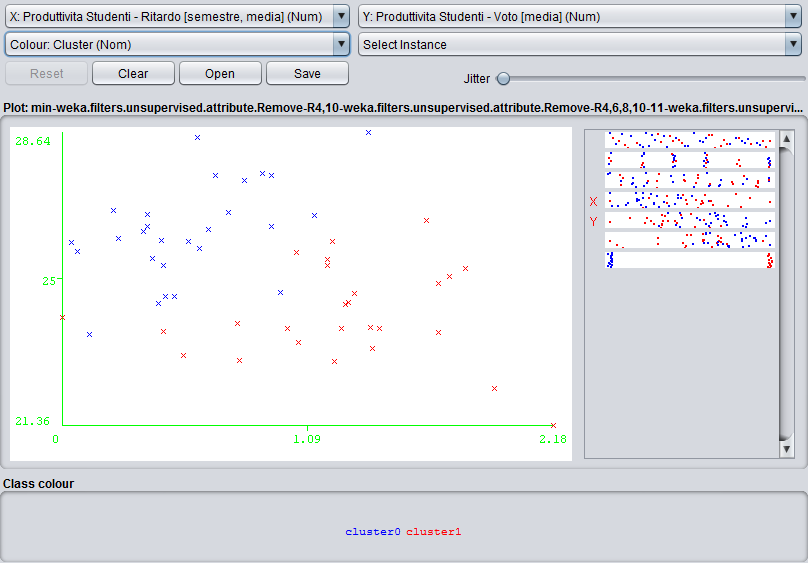
\includegraphics[scale=0.5]{../cluster/min_kmeans_2cl_attr1.png}
        \end{figure}

        \begin{figure}
            \centering
            \caption{sezione dello spazio di esistenza del data set delle valutazione dei corsi lungo il piano definito da "ritardo medio" e "valutazione della didattica", con evidenziato per ogni istanza il cluster di appartenenza}
            \label{2}
            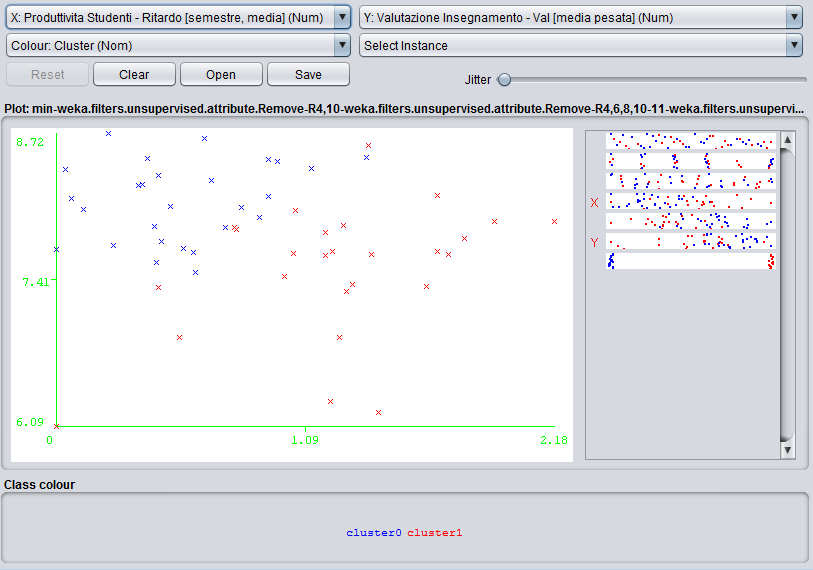
\includegraphics[scale=0.5]{../cluster/min_kmeans_2cl_attr2.png}
        \end{figure}

        \begin{figure}
            \centering
            \caption{sezione dello spazio di esistenza del data set delle valutazione dei corsi lungo il piano definito da "voto medio" e "valutazione della didattica", con evidenziato per ogni istanza il cluster di appartenenza}
            \label{3}
            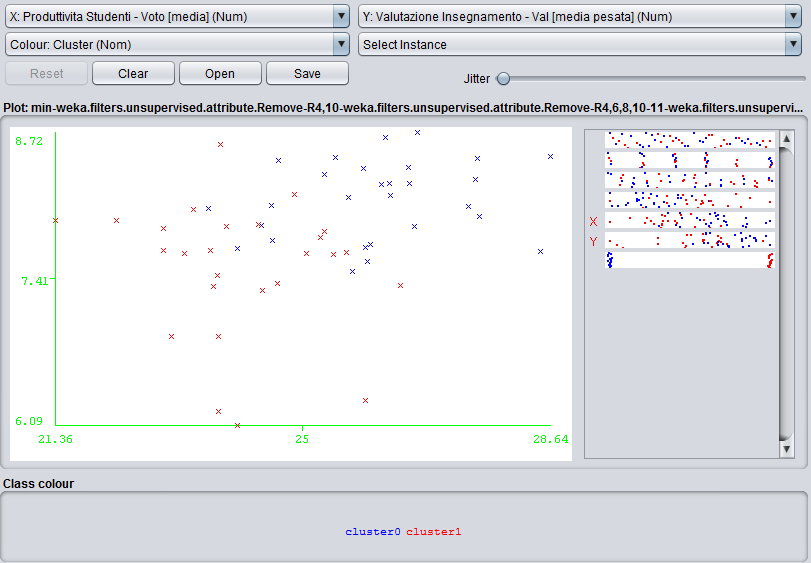
\includegraphics[scale=0.5]{../cluster/min_kmeans_2cl_attr3.png}
        \end{figure}

        Volendo ragionare sulla composizione dei due cluster, si è andati a vedere innanzitutto se l'Anno Accademico di riferimento ha un qualche ruolo nella produzione di questo risultato. Come si può osservare nelle Figure \ref{AA1} e \ref{AA2}, la popolazione di entrambi i cluster è abbastanza simile riguardo a questo aspetto. \\

        \begin{figure}
            \centering
            \caption{composizione del Cluster $0$ riguardo gli Anni Accademici considerati dal data set}
            \label{AA1}
            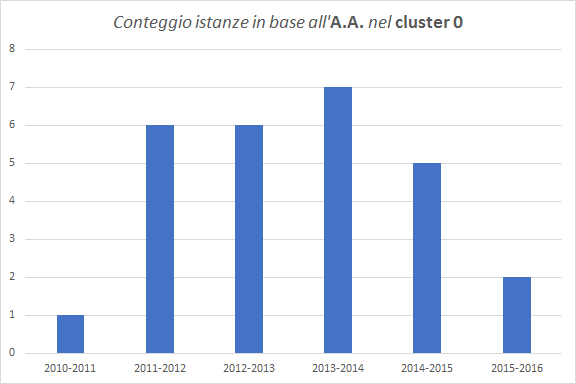
\includegraphics[scale=0.75]{../cluster/min_kmeans_2cl_AA_cl0.png}
        \end{figure}

        \begin{figure}
            \centering
            \caption{composizione del Cluster 1 riguardo gli Anni Accademici considerati dal data set}
            \label{AA2}
            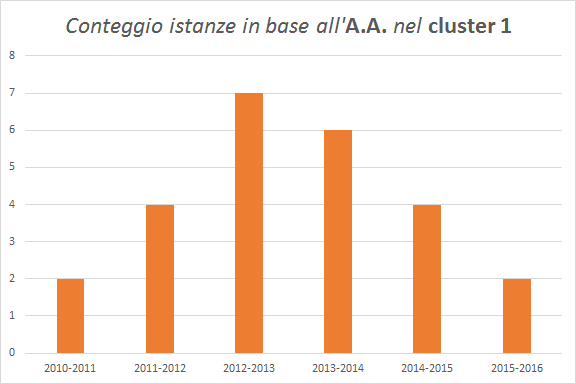
\includegraphics[scale=0.75]{../cluster/min_kmeans_2cl_AA_cl1.png}
        \end{figure}

        Per quanto riguarda invece l'individuare quali corsi sono finiti in quale cluster, si è innanzitutto osservata la composizione totale dei due cluster. In caso si fosse trattato di una \textit{cluster analysis} su veri e propri \textit{big data}, questo non sarebbe ovviamente stato possibile, ma dato che il data set in esame ha a malapena sessanta istanze, è stato possibile stilare la seguente lista: \\

        \lstinputlisting{../cluster/min_kmeans_2cl_composition.txt}

        Tuttavia, tale lista non consente di vedere immediatamente alcuna caratteristica fondamentale del clustering in esame. La maggior parte dei corsi, rappresentati da varie istanze secondo l'Anno Accademico di riferimento, è presente sia nel Cluster $0$ che nel Cluster 1. Pertanto, è stata realizzata la tabella mostrata in Figura \ref{tabella} per evidenziare quali corsi di esame sono del tutto assenti da quali cluster.\\

        \begin{figure}
            \centering
            \caption{tabella che mostra la composizione dei cluster in riferimento ai corsi di esame}
            \label{tabella}
            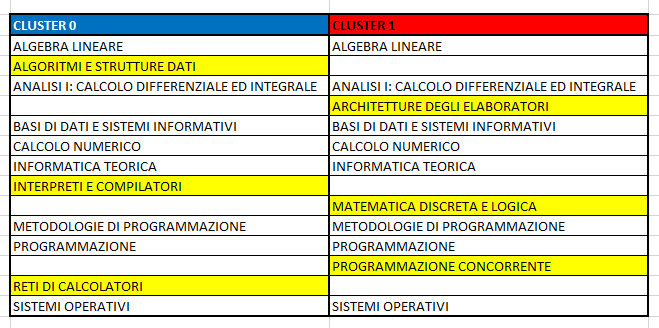
\includegraphics[scale=0.65]{../cluster/min_kmeans_2cl_corsi_cluster.png}
        \end{figure}

        Da tale Figura, si può notare che il Cluster $0$, quello dei corsi "buoni", comprende tutte le istanze relative ai corsi di:

        \begin{itemize}
            \item Algoritmi e Strutture dati
            \item Interpreti e Compilatori
            \item Reti di Calcolatori
        \end{itemize}

        Inoltre, si può vedere che nel Cluster 1, quello dei corsi "meno buoni", sono presenti tutte le istanze dei seguenti corsi:

        \begin{itemize}
            \item Architetture degli Elaboratori
            \item Matematica Discreta e Logica
            \item Programmmazione Concorrente
        \end{itemize}

        Questa caratteristica richiama fortemente quanto visto nel Capitolo \ref{ch:undst}, ovvero durante la fase di \textit{data understanding}, rafforzando quindi l'ipotesi della bontà dell'analisi che si sta effettuando. \\

        Volendo approfondire ulteriormente l'analisi della composizione dei cluster, nelle Figure \ref{eval}, \ref{ritardo} e \ref{voto} si possono vedere degli istogrammi che mostrano la somma dei tre attributi considerati per realizzare il clustering. Ovviamente, i valori assoluti di tali somme non significano niente, ma è interessante vedere come gli attributi "positivi" --- la valutazione della didattica e il voto medio --- hanno una somma più elevata nel Cluster $0$, mentre quello "negativo" --- il ritardo nel dare gli esami --- è molto più accentuato nel Cluster 1.

        \begin{figure}
            \centering
            \caption{istogramma che mostra la somma dell'attributo "valutazione della didattica" nei due cluster ottenuti, divisa per Anno Accademico}
            \label{eval}
            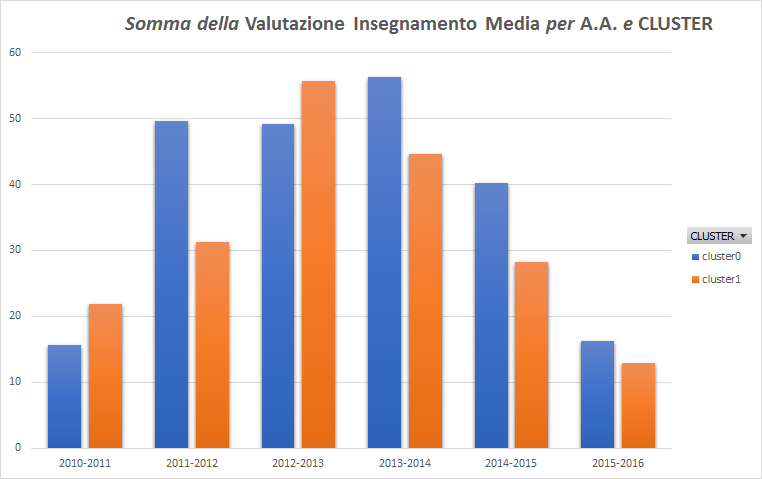
\includegraphics[scale=0.5]{../cluster/min_kmeans_2cl_eval.png}
        \end{figure}

        \begin{figure}
            \centering
            \caption{istogramma che mostra la somma dell'attributo "ritardo medio nel dare gli esami" nei due cluster ottenuti, divisa per Anno Accademico}
            \label{ritardo}
            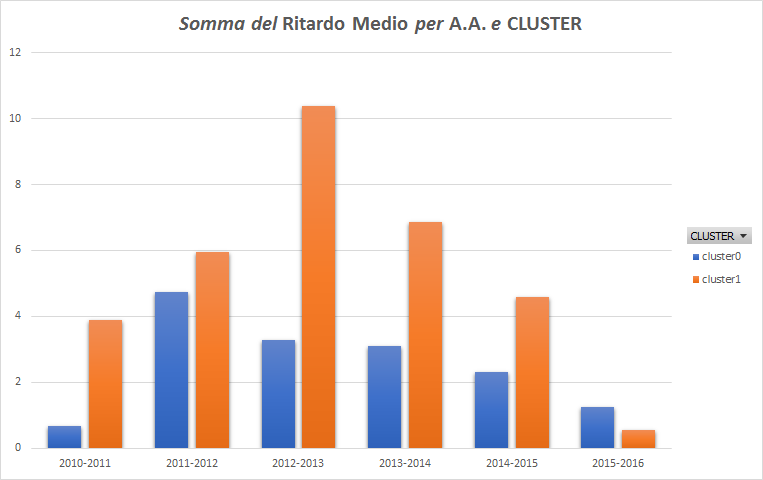
\includegraphics[scale=0.5]{../cluster/min_kmeans_2cl_ritardo.png}
        \end{figure}

        \begin{figure}
            \centering
            \caption{istogramma che mostra la somma dell'attributo "voto medio conseguito all'esame" nei due cluster ottenuti, divisa per Anno Accademico}
            \label{voto}
            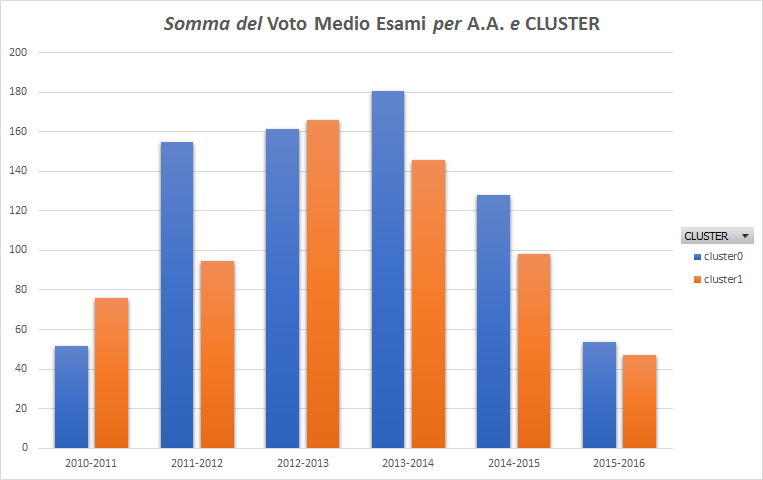
\includegraphics[scale=0.5]{../cluster/min_kmeans_2cl_voto.png}
        \end{figure}

    \subsection{Tentativo di utilizzo di DBSCAN}

    Come il titolo di questa sezione suggerisce, non è stato possibile utilizzare con profitto l'algoritmo DBSCAN. \\

    Imitando quanto fatto con K-Means, ovvero limitando il numero di attributi da considerare per il clustering, ci si aspetterebbe che un algoritmo basato sulla densità possa esibire delle buone performance. Per facilitare ulteriormente l'esecuzione di DBSCAN, è stato addirittura scartato l'attributo relativo al ritardo degli studenti. Così facendo, si è ottenuto uno spazio bidimensionale in cui l'algoritmo può facilmente operare - e che si presta bene a una interpretazione visiva. \\

    Invece, non è stato possibile ottenere nessun risultato diverso da un cluster unico, per qualunque valore di epsilon e per qualsiasi numero di punti minimi richiesti. Questo perché evidentemente i punti nel nostro piano di analisi sono addensati tutti in un'unica regione, fatto che possiamo agilmente verificare osservandone un grafico in Figura \ref{dbscan}.

    \begin{figure}
        \centering
        \caption{piano composto dalle dimensioni "Voto Medio negli Esami" e "Valutazione Media dell'Insegnamento", sul quale è stato tentato il clustering con l'algoritmo DBSCAN}
        \label{dbscan}
        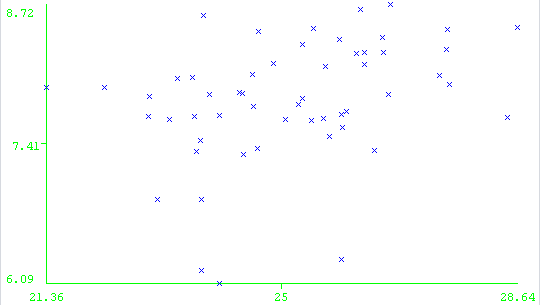
\includegraphics[scale=0.75]{../cluster/dbscan.png}
    \end{figure}
\begin{frame}{Frequent Sequential Patterns}{Looking for meaningful frequent patterns in exams sequences}

    \centering\textit{Which exams are "skipped" the most by the students?} \vspace{0,3cm}

\begin{block}{Mining process}
		\begin{itemize}
			\item<1-> \alert{GSP algorithm} --- Apriori-based algorithm to extract frequent sequential patterns from the \emph{students} data set;
			\item<2-> \alert{Unusual pattern mining} --- filtering of the GSP output, with the goal of discarding uninteresting (regular) exams patterns;
			\item<3-> \alert{Out-of-place exams mining} --- extraction of the exams that are passed \emph{after} a later exam.
		\end{itemize}
	\end{block}

\end{frame}


\begin{frame}{Associative Rules Analysis}{Looking for implications among the dataset's attributes}

    \alert{Example} of a frequent, unusual pattern: \\

	\vspace{0.3cm}
	\begin{centering}\texttt{Calcolo Numerico, Informatica Teorica, Fisica Generale}\end{centering} \\
	\vspace{0.3cm}

	\texttt{Fisica Generale} is out of place, for it is a $2^{nd}$ year exam done after some $3^r{d}$ year exams.\\

\end{frame}
\chapter{Analisi Associativa}
\label{ch:ass}

Di seguito verrà descritto il lavoro svolto nell'ambito della ricerca di regole associative. \\

Come è già stato accennato in precedenza, questo tipo di analisi ha richiesto l'impiego delle versioni discretizzate dei data set provenienti dalla fase di \textit{preprocessing}. Il motivo di questo requisito apparirà chiaro andando a descrivere brevemente il funzionamento delle tecniche di analisi associativa.

\section{Introduzione all'analisi associativa}

    Questa introduzione vuole essere solo un breve riassunto dei concetti fondamentali seguiti per realizzare all'atto pratico l'analisi. Una trattazione più approfondita --- che trascenderebbe  ampiamente lo scopo di questa tesi di laurea --- può essere trovata in \cite{dispense}, ed è proprio quella che è stata consultata per realizzare quanto segue.

    \subsection{Regole Associative}

        Una regola associativa è una implicazione del tipo $A \rightarrow B$, con $A$ e $B$ insiemi di item (detti, appunto \textit{itemset}). Il significato di ciò dovrebbe essere palese: data la presenza di $A$ in una istanza del data set, è \textit{fortemente probabile} la presenza di $B$. La valutazione di questa probabilità avviene considerando alcune metriche particolari quali, ad esempio, la \textit{confidenza} o il \textit{lift}. \\

        Portando un esempio sul data set oggetto di questa analisi, una tanto probabile quanto banale regola associativa che ci si aspetta di trovare potrà essere del tipo \textit{"Valutazione del corso: ALTA"} $\rightarrow$ \textit{"Voto conseguito: ALTO"}. \\

        Quello a cui si mira, però, è riuscire a scoprire qualche altra regola che trascenda il limite dell'ovvio, aprendo così le porte a interpretazioni non immediate dell'insieme di dati su cui si sta lavorando. Per questo motivo, oltre all'aiuto di criteri algoritmici di potatura, occorrerà comunque prevedere un \textit{intervento umano} nel \textit{post processing} delle regole generate.

    \subsection{L'algoritmo Apriori di Weka}

    \begin{figure}
        \centering
        \caption{pannello di scelta delle impostazioni per l'algoritmo Apriori di Weka}
        \label{apriori_weka}
	    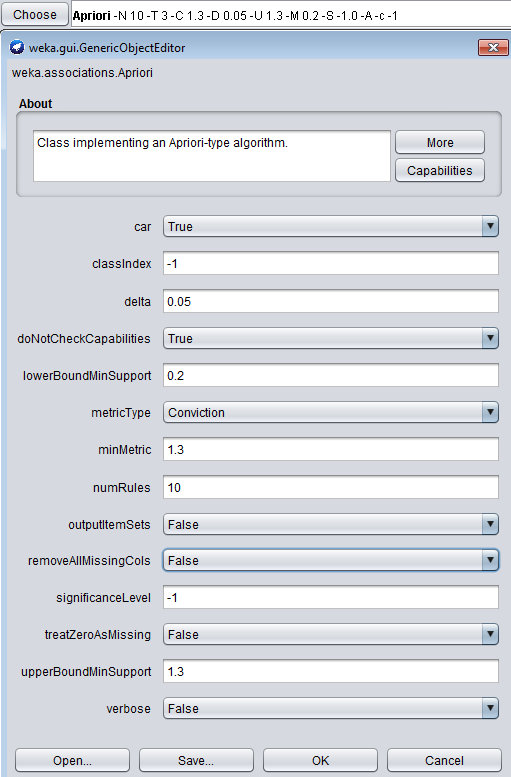
\includegraphics[scale=1.0]{img/apriori_weka.png}
    \end{figure}

        Il processo di generazione delle regole associative utilizzato in questa analisi si basa sul \textbf{principio Apriori}. Dato che una regola non è altro che una implicazione generata da un partizionamento binario di un itemset frequente, il pilastro fondamentale da cui partire per generare le regole è il \textit{mining} degli itemset frequenti. \\

        In estrema sintesi, l'idea generale è quella di generare una lista di \textit{candidati} semplici --- cioè di itemset che potrebbero essere frequenti --- verificarne il \textit{supporto} e usare quelli idonei per generare altri candidati più complessi. Il principio Apriori, infatti, stabilisce che se un itemset con pochi elementi è infrequente, lo saranno anche tutti gli itemset che lo comprendono. Questo fatto, detto \textit{anti-motonia} del supporto, ci consente di evitare di generare e calcolare la frequenza di ogni possibile itemset, rendendo trattabile quello che sarebbe invece un problema $NP-Completo$. \\

        Nel dettaglio dell'analisi da effettuare, l'algoritmo Apriori messo a disposizione dal software Weka accetta in input diversi parametri, che consentono di specificarne il comportamento dell'algoritmo, adattandolo agli scopi che ci si è prefissi. Si veda adesso una configurazione di esempio:\\

        \begin{center}
            \noindent \texttt{Apriori -N 10 -T 0 -C 0.9 -D 0.05 -U 1.0 -M 0.1}
        \end{center}

        I vari \textit{flags} da passare come argomenti vanno a regolare questi parametri della computazione:

        \begin{itemize}
            \item \texttt{-N}: numero di regole associative da trovare;
            \item \texttt{-T}: tipo di metrica utilizzata per la valutazione degli itemset
                \subitem 0 - \textit{confidence}
                \subitem 1 - \textit{lift}
                \subitem 2 - \textit{leverage}
                \subitem 3 - \textit{convction};
            \item \texttt{-C}: valore minimo della metrica indicata per considerare frequente un itemset;
            \item \texttt{-D}: valore che viene usato per diminuire il supporto ad ogni iterazione dell'algoritmo;
            \item \texttt{-U}: limite superiore del supporto minimo richiesto;
            \item \texttt{-M}: limite inferiore del supporto minimo richiesto.
        \end{itemize}

        Ovviamente, come si può vedere in Figura \ref{apriori_weka}, sono possibili molte altre personalizzazioni e impostazioni, fatto che rende l'implementazione di Weka dell'algoritmo Apriori estremamente flessibile ed adattabile a molte esigenze. \\

\section{Apriori su dataset aggregato}

    Decidere a priori i parametri ottimali per l'algoritmo Apriori\footnote{gioco di parole \textbf{non} intenzionale.} è da considerarsi impossibile. Pertanto, anche in questo caso l'iter più adatto per ottenere dei risultati che possono essere giudicati interessanti è il banale ma efficace \textit{trial-and-error}. \\

    La conseguenza immediata di questo è che, similarmente a quanto fatto per la descrizione di altri tipi di analisi sui dati, in questa sezione verranno riportati solo gli output giudicati in qualche senso significativi. \\

    In ogni caso, alcune scelte sono state comuni a tutte le analisi:

    \begin{itemize}
        \item come \textit{metrica} è stato scelto il \textbf{Lift}, un cui valore positivo indica una correlazione effettiva --- cosa che non è affatto garantita da un alto valore di \textit{confidenza};
        \item non è stata usata la valutazione per classe, né il pruning per livello di significato;
        \item sono stati sempre stampati gli itemset frequenti, in quanto utili per capire l'andamento della generazione delle regole;
        \item come \textit{delta} è stato scelto un valore il più piccolo possibile, ma compatibile con dei tempi macchina "umani".
    \end{itemize}

        \subsection{Focus sul corso}

            L'analisi che viene presentata nel'immediato seguito è stata ottenuta cercando correlazioni fra gli attributi relativi all'andamento generale dei corsi d'esame. In particolare, oltre che verificare, come ipotizzato, la presenza di regole del tipo \textit{"Valutazione del corso: ALTA"} $\rightarrow$ \textit{"Voto conseguito: ALTO"}, andare a vedere se esistono legami fra questi due aspetti e il ritardo con cui uno studente supera un esame. \\

            L'algoritmo è stato lanciato sul data set \texttt{min\_d.csv}, ulteriormente semplificato grazie alla considerazione di questi soli attributi:

            \begin{itemize}
                \item identificativo dell'insegnamento;
                \item ritardo medio del superamento dell'esame (rispetto al primo appello disponibile, contato in semestri);
                \item voto medio ottenuto all'esame dagli studenti;
                \item valutazione media del corso d'insegnamento.
            \end{itemize}

            Il miglior risultato che si è ottenuto in quest'ottica è il seguente: \\

            \lstinputlisting{../ass/apriori_min_1.txt}

            \begin{figure}
                \centering
                \caption{visualizzazione 3D delle regole assciative trovate con focus sul corso}
                \label{apriori_min_1}
	            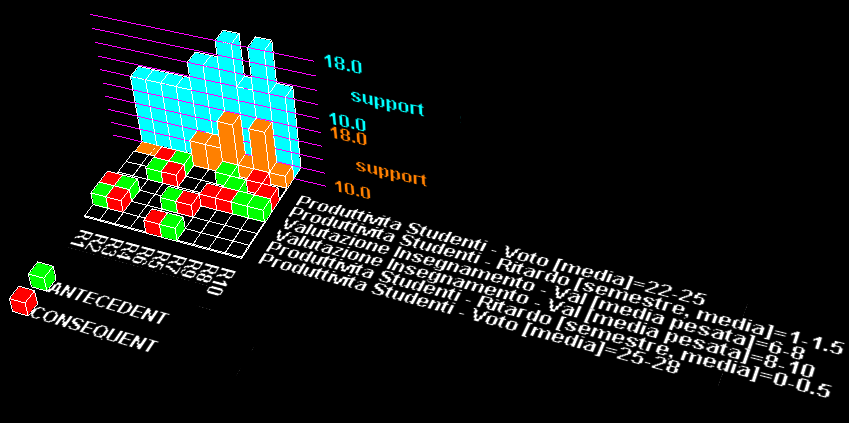
\includegraphics[scale=0.48]{../ass/apriori_min_1.png}
            \end{figure}

            Semplificando la \textit{naming convention} a favore della leggibilità, le regole trovate sono queste:

            \begin{itemize}
                \item \textbf{R1}: Ritardo: $BASSO$ $\rightarrow$ Valutazione insegnamento: $OTTIMA$
                \item \textbf{R2}: Valutazione insegnamento: $OTTIMA$ $\rightarrow$ Ritardo: $BASSO$
                \item \textbf{R3}: Ritardo: $ALTO$ $\rightarrow$ Voto: $MEDIO-BASSO$
                \item \textbf{R4}: Voto: $MEDIO-BASSO$ $\rightarrow$ Ritardo: $ALTO$
                \item \textbf{R5}: Voto: $MEDIO-ALTO$ $\rightarrow$ Valutazione insegnamento: $OTTIMA$
                \item \textbf{R6}: Valutazione insegnamento: $OTTIMA$ $\rightarrow$ Voto: $MEDIO-ALTO$
                \item \textbf{R7}: Voto: $MEDIO-BASSO$ $\rightarrow$ Valutazione insegnamenti: $SUFF.$
                \item \textbf{R8}: Valutazione insegnamenti: $SUFF.$ $\rightarrow$ Voto: $MEDIO-BASSO$
                \item \textbf{R9}: Ritardo: $ALTO$ $\rightarrow$ Valutazione insegnamenti: $SUFF.$
                \item \textbf{R10}: Valutazione insegnamenti: $SUFF.$ $\rightarrow$ Ritardo: $ALTO$
            \end{itemize}

            Andando ad analizzare le regole trovate, eliminando ridondanze ed effettuando una sorta di \textit{post processing} manualmente, le informazioni chiave che si sono ottenute risultano essere le seguenti:

            \begin{itemize}
                \item Ritardo: $BASSO$ $\leftarrow \rightarrow$ Valutazione insegnamento: $OTTIMA$
                \item Ritardo: $ALTO$ $\leftarrow \rightarrow$ Voto: $MEDIO-BASSO$
                \item Ritardo: $ALTO$ $\leftarrow \rightarrow$ Valutazione insegnamenti: $SUFF.$
                \item Voto: $MEDIO-ALTO$ $\leftarrow \rightarrow$ Valutazione insegnamento: $OTTIMA$
                \item Voto: $MEDIO-BASSO$ $\leftarrow \rightarrow$ Valutazione insegnamenti: $SUFF.$
            \end{itemize}

            Quelle trovate sono \underline{tutte} implicazioni doppie, il che significa che fra gli attributi esiste una forte correlazione. Messa da parte l'attesa e apparente proporzionalità diretta fra la valutazione del corso e il voto ottenuto all'esame, si può notare l'esistenza di una analoga correlazione fra il ritardo con cui gli studenti hanno superato l'esame e la valutazione del corso.

        \subsection{Focus sul docente}

            Facendo uso di alcuni, specifici attributi del dataset \texttt{full\_d.csv}, si è tentato di scoprire correlazioni fra la produttività degli studenti e l'aspetto della valutazione del corso relativo al docente. Nel particolare, sono stati considerati questi attributi:

            \begin{itemize}
                \item Identificativo del docente
                \item Ritardo medio del superamento dell'esame
                \item Voto medio ottenuto all'esame dagli studenti
                \item Valutazione media del paragrafo relativo al docente
            \end{itemize}

            Il miglior risultato che si è ottenuto, a seguito di iterazioni volte a proseguire nella direzione sopra descritta, è il seguente: \\

            \lstinputlisting{../ass/apriori_min_2.txt}

            \begin{figure}
                \centering
                \caption{visualizzazione 3D delle regole assciative trovate con focus sul docente}
                \label{apriori_min_2}
	            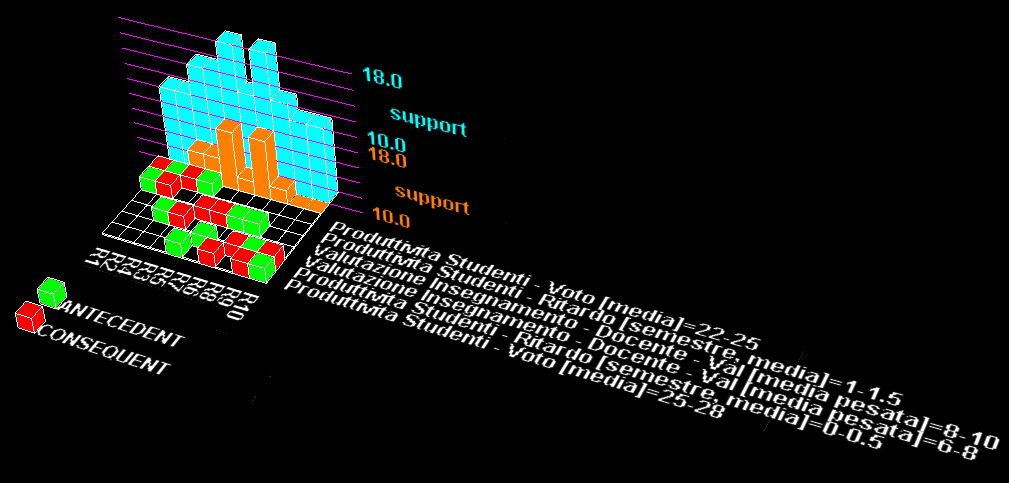
\includegraphics[scale=0.4]{../ass/apriori_min_2.png}
            \end{figure}

            Scartando immediatamente le regole già ottenute nell'analisi precedente --- quelle relative alle correlazioni fra il ritardo nel superamento e il voto all'esame --- si consideri la seguente sintesi delle regole trovate:

            \begin{itemize}
                \item Voto medio-basso $\leftarrow \rightarrow$ Valutazione docente sufficiente
                \item Voto medio-alto $\leftarrow \rightarrow$ Valutazione docente ottima
                \item Ritardo basso $\leftarrow \rightarrow$ Valutazione docente ottima
            \end{itemize}

            La correlazione fra la valutazione del docente e i risultati ottenuti appare molto forte, ma purtroppo è anche del tutto analoga a quella fra i risultati e la valutazione generale del corso.

        \subsection{Focus sulla Deviazione Standard}

        Nel data set \texttt{min\_d.csv} sono state mantenute informazioni complementari rispetto alle medie pesate dei valori che hanno composto l'aggregazione, quali ad esempio lo scarto quadratico medio di un certo attributo. Gli attributi contenenti questi dati sono stati ignorati nelle due precedenti analisi associative, pertanto è sembrato interessante andate a vedere se esiste una qualche regola fra i seguenti parametri:

            \begin{itemize}
                \item Hash del docente
                \item Identificativo dell'insegnamento
                \item Percentuale di studenti il cui ritardo nel dare un certo esame supera il semestre
                \item Percentuale di studenti il cui voto conseguito in un dato esame supera il 24
                \item Deviazione standard dei voti ottenuti dagli studenti in quell'esame
                \item Media delle deviazioni standard delle valutazioni dell'insegnamento nei vari paragrafi
                \item Media delle percentuali di valutazioni dell'insegnamento sufficienti  
            \end{itemize}

            \lstinputlisting{../ass/apriori_min_3.txt}

            Non ci si aspettava di trovare niente di particolarmente significativo riguardo qusti aspetti del data set. Invece, sono comparse due regole associative che possiamo riassumere in una implicazione doppia come segue:

            \begin{center}
                \textbf{R1}: Deviazione standard del voto: MOLTO GRANDE $\leftarrow \rightarrow$ Deviazione standard della valutazione dell'insegnamento: GRANDE
            \end{center}

            Si tratta di una associazione forte, in quanto le due regole che la compongono hanno entrambe una confidenza abbastanza elevata --- R1: 0.8, R2: 0.68 --- ed un valore del lift sì minimo, ma comunque positivo. \\

\section{Conclusioni}

    Volendo riassumere quanto notato dai risultati delle analisi effettuate, si può affermare quanto segue:

    eh, tbd
\chapter{Conclusioni e Futuri Sviluppi}
\label{ch:fine}

Dopo aver ampiamente esposto e illustrato tutto il lavoro fatto, non resta che trare una sintesi conclusiva. \\

Quanto è stato portato alla luce dalle varie attività di \textit{data mining} che sono state svolte rapprsenta sicuramente soltanto una minima parte delle informazioni preziosamente racchiuse nella mole di dati scelta come base. Ci si può comunque definire soddisfatti di quanto ottenuto, in quanto esaurire la "miniera" in quest'unica occasione non è mai stato l'obiettivo prefisso: al contrario, ciò che ha reso importante questa serie di analisi è stata la possibilità di affinare l'intuito e la fantasia necessaria al \textit{data scientist} per poter svolgere efficacemente il suo lavoro.\\

Non si presenteranno tesi o speculazioni in merito alle implicazioni di quanto estratto, in questa sede: ciò trascenderebbe lo scopo dell'intera tesi e la competenza dell'autore. Si è certi però che questo lavoro possa essere una base di partenza per ulteriori approfondimenti, che potranno fornire un solido supporto per scoprire le cause di alcuni degli aspetti relativi a quanto studiato. \\

Magari, proseguendo per questa strada, si riuscirà a portare un concreto miglioramento al Corso di Laurea in Informatica.
\begin{thebibliography}{99}

    \bibitem{mongodb}{\url{https://docs.mongodb.com/manual/} --- \emph{The MongoDB 3.6 Manual} --- MongoDB, Inc}

    \bibitem{mongowiki}{\url{https://it.wikipedia.org/wiki/MongoDB} --- \emph{MongoDB} --- Wikipedia, l'enciclopedia libera}

    \bibitem{pymongo}{\url{https://api.mongodb.com/python/3.6.0/} --- \emph{PyMongo 3.6.0 Documentation} --- MongoDB, Inc}

    \bibitem{python}{\url{https://docs.python.org/3.6/} --- \emph{Python 3.6.6rc1 Documentation} --- Python Software Foundation}

    \bibitem{pywiki}{\url{https://it.wikipedia.org/wiki/Python} --- \emph{Python} --- Wikipedia, l'enciclopedia libera}

    \bibitem{make}{\url{https://www.gnu.org/software/make/} --- \emph{GNU Make} --- Free Software Foundation}

    \bibitem{weka}{\url{https://www.cs.waikato.ac.nz/ml/weka/documentation.html} --- \emph{WEKA Manual for Version 3-8-2} --- Machine Learning Group at the University of Waikato}

    \bibitem{wekawiki}{\url{https://it.wikipedia.org/wiki/Weka} --- \emph{Weka} --- Wikipedia, l'enciclopedia libera}

    \bibitem{R}{\url{https://cran.r-project.org/manuals.html} --- \emph{The R Manuals} --- The R Foundation}

    \bibitem{Rwiki}{\url{https://it.wikipedia.org/wiki/R_(software)} --- \emph{R (software)} --- Wikipedia, l'enciclopedia libera}

    \bibitem{calc}{\url{https://documentation.libreoffice.org/en/} --- \emph{Calc Guide} --- Libre Office, The Document Foundation}

    \bibitem{articolo}{\emph{An Analysis of Courses Evaluation Through Clustering} --- Renza Campagni, Donatella Merlini, Maria Cecilia Verri}

    \bibitem{dispense}{\emph{Introduction to Data Mining} --- Pang-Ning Tan, Michael Steinbach, Vipin Kumar}

    \bibitem{clustering}{\url{https://it.wikipedia.org/wiki/Clustering} --- \emph{Clustering} --- Wikipedia, l'enciclopedia libera}

    \bibitem{pragmatic}{\emph{The Pragmatic Programmer: From Journeyman to Master} --- Andrew Hunt, David Thomas}

\end{thebibliography}

%--------------------------------------------------------------
\end{document}

